\documentclass[12pt, twoside]{book}

% Document Preamble: basic definitions and packages.
\usepackage[english]{babel}
\usepackage[utf8]{inputenc}

% Page Margins and General Spacing
\usepackage[top=2.5cm, left=2cm, right=2cm, bottom=2.0cm]{geometry}
\usepackage{setspace}
\usepackage{xspace}

% References and \url
\usepackage{hyperref}

% Math-mode Coolness
\usepackage{amsmath}

% Custom Name Abbreviations
\newcommand{\projName}{\textsc{MedSpark}\xspace}
\newcommand{\sgxspark}{\textsc{SGX-Spark}\xspace}
\newcommand{\sgx}{\textsc{SGX}\xspace}
\newcommand{\tz}{\textsc{TrustZone}\xspace}
\newcommand{\arm}{\textsc{Arm}\xspace}

% Graphics and TiKz
\usepackage{graphicx}
\usepackage{wrapfig} % Wrapping figures w/ text
\usepackage{tikz}
\usetikzlibrary{decorations.pathmorphing, patterns}
% We use this commands for sgx-principles.tex figure
\usepackage{pifont} % To use circled numbers in text
\newcommand*\blackcircled[1]{\tikz[baseline=(char.base)]{
            \node[shape=circle,fill,inner sep=0.5pt] (char) {\textcolor{white}{#1}};}}
\newcommand*\circled[1]{\tikz[baseline=(char.base)]{
            \node[shape=circle,draw,inner sep=2pt] (char) {#1};}}

% Headers, Footers and page numeration
\usepackage{fancyhdr}
% This is currently the default, change when placeholders TODO
%\fancyhead[LE,RO]{\slshape \rightmark}
%\fancyhead[LO,RE]{\slshape \leftmark}
%\fancyfoot[C]{\thepage}
%\pagestyle{fancy}
\fancypagestyle{frontmatter}{% Pagestyle for the frontmatter
  \renewcommand{\headrulewidth}{0pt}% No header rule
  \renewcommand{\footrulewidth}{0pt}% No footer rule
  \fancyhf[R]{\thepage}% Top right page number
  \fancyfoot{}%
}
\fancypagestyle{mainmatter}{%
  \renewcommand{\headrulewidth}{.4pt}% Header rule
  \renewcommand{\footrulewidth}{.0pt}% Footer rule
  %\fancyhf{}% Clear header/footer
  \fancyhead[LE]{\slshape\nouppercase{\leftmark}}% Chapter in header Left
  \fancyhead[RE]{\thepage}% Page number in header Right
  \fancyhead[LO]{\thepage}% Chapter in header Left
  \fancyhead[RO]{\slshape\nouppercase{\rightmark}}% 
  \fancyfoot{}
}
% The plain pagestyle is the one used by new Chapter pages and the ToC
\fancypagestyle{plain}{%
  \fancyhf{}%
  \fancyhead[R]{\thepage}
  \fancyfoot{}%
  \renewcommand{\headrulewidth}{0pt}% Line at the header invisible
  \renewcommand{\footrulewidth}{0pt}% Line at the footer visible
}

% Epigraph Package (Book Citation)
\usepackage{epigraph}
\setlength\epigraphwidth{.5\textwidth}

% Placeholders
\usepackage{lipsum}

% List of acronyms
\usepackage[toc,acronym,nomain,nonumberlist]{glossaries}

% Appendices
\usepackage[titletoc]{appendix}

% Code Listings Configuration
\usepackage{listings}
\definecolor{backcolour}{rgb}{0.95,0.95,0.92}
\lstset{ 
  backgroundcolor=\color{backcolour},   % Background color
  basicstyle=\footnotesize,        % the size of the fonts that are used for the code
  breakatwhitespace=false,         % sets if automatic breaks should only happen at whitespace
  breaklines=true,                 % sets automatic line breaking
  captionpos=b,                    % sets the caption-position to bottom
  commentstyle=\color{gray},    % comment style
  deletekeywords={...},            % if you want to delete keywords from the given language
  escapeinside={\%*}{*)},          % if you want to add LaTeX within your code
  extendedchars=true,              % lets you use non-ASCII characters; for 8-bits encodings only, does not work with UTF-8
  firstnumber=1,                % start line enumeration with line 1000
  frame=trbl,	                   % adds a frame around the code
  keepspaces=true,                 % keeps spaces in text, useful for keeping indentation of code (possibly needs columns=flexible)
  keywordstyle=\color{blue},       % keyword style
  morekeywords={*,println},            % if you want to add more keywords to the set
  numbers=left,                    % where to put the line-numbers; possible values are (none, left, right)
  numbersep=5pt,                   % how far the line-numbers are from the code
  numberstyle=\tiny\color{gray!80}, % the style that is used for the line-numbers
  rulecolor=\color{black},         % if not set, the frame-color may be changed on line-breaks within not-black text (e.g. comments (green here))
  showspaces=false,                % show spaces everywhere adding particular underscores; it overrides 'showstringspaces'
  showstringspaces=false,          % underline spaces within strings only
  showtabs=false,                  % show tabs within strings adding particular underscores
  stepnumber=1,                    % the step between two line-numbers. If it's 1, each line will be numbered
  stringstyle=\color{purple},     % string literal style
  tabsize=2,	                   % sets default tabsize to 2 spaces
  title=\lstname                   % show the filename of files included with \lstinputlisting; also try caption instead of title
}
% Syntax Highlighting for Scala
\lstdefinelanguage{Scala}{
  morekeywords={%
          abstract,case,catch,class,def,do,else,extends,%
          false,final,finally,for,forSome,if,implicit,import,lazy,%
          match,new,null,object,override,package,private,protected,%
          return,sealed,super,this,throw,trait,true,try,type,%
          val,var,while,with,yield},
  otherkeywords={=>,<-,<\%,<:,>:,\#,@},
  sensitive=true,
  morecomment=[l]{//},
  morecomment=[n]{/*}{*/},
  morestring=[b]",
  morestring=[b]',
  morestring=[b]"""
}[keywords,comments,strings]
% Syntax Highlighting for Dockerfiles
\lstdefinelanguage{Dockerfile}{
  morekeywords={FROM, RUN, CMD, LABEL, MAINTAINER, EXPOSE, ENV, ADD, COPY,
    ENTRYPOINT, VOLUME, USER, WORKDIR, ARG, ONBUILD, STOPSIGNAL, HEALTHCHECK,
    SHELL},
  morecomment=[l]{\#},
  morestring=[b]"
}
% Syntax Highlighting for Docker Compose files
\lstdefinelanguage{docker-compose}{
  keywords={image, environment, ports, container_name, ports, volumes, links},
  keywordstyle=\color{blue}\bfseries,
  identifierstyle=\color{black},
  sensitive=false,
  comment=[l]{\#},
  commentstyle=\color{purple}\ttfamily,
  stringstyle=\color{red}\ttfamily,
  morestring=[b]',
  morestring=[b]"
}
\renewcommand\lstlistlistingname{List of Listings}


% List of acronyms
\makeglossaries
\newacronym{api}{API}{Application Programing Interface}
\newacronym{dft}{DFT}{Discrete Fourier Transform}
\newacronym{dsm}{DSM}{Data Stream Manager}
\newacronym{ecg}{ECG}{Electrocardiogram}
\newacronym{hr}{HR}{Heart Rate}
\newacronym{hrv}{HRV}{Heart Rate Variability}
\newacronym{iaas}{IaaS}{Infrastructure-as-a-Service}
\newacronym{loc}{LoC}{Lines of Code}
\newacronym{lsds}{LSDS}{Large Scale Data \& Systems}
\newacronym{jvm}{JVM}{Java Virtual Machine}
\newacronym{mee}{MEE}{Memory Encryption Engine}
\newacronym{os}{OS}{Operating System}
\newacronym{ppg}{PPG}{Photoplethysmogram}
\newacronym{rhs}{RHS}{Right Hand Side}
\newacronym{sgx}{SGX}{Software Guard eXtensions}
\newacronym{sftp}{SFTP}{Secure File Transfer Protocol}
\newacronym{shm}{SHM}{Shared Memory}
\newacronym{sshfs}{SSHFS}{Secure SHell File System}
\newacronym{ta}{TA}{Trusted Application}
\newacronym{tee}{TEE}{Trusted Execution Environment}
\newacronym{tls}{TLS}{Transport Layer Security}
\newacronym{unine}{UniNe}{University of Neuch\^atel}
\newacronym{vmm}{VMM}{Virtual Machine Monitor}




\begin{document}
\onehalfspacing

\frontmatter
\pagestyle{frontmatter}

% Title page
\thispagestyle{empty}
\begin{center}

    % FME - ETSETB
    
\includegraphics[width=8cm]{img/logo-fme.png} 
    \hfill
    
\includegraphics[width=9cm]{img/logo-upc.png}

    \vspace{0.5cm}

    % Joint work mention CFIS
    \Large
    \textsc{Joint Bachelor Thesis in Mobile} 

    \textsc{Interdisciplinary Higher Education Center (CFIS-UPC)}

    % Thesis Title
    \LARGE
    \rule{\textwidth}{0.4pt}
    \textbf{\projName: Using Trusted Execution Environments for Secure Stream Processing of Medical Data}
    \rule[0.5cm]{\textwidth}{0.4pt}

    % Semester
    \vspace{-0.2cm}
    \Large
    \textsc{Autumm Semester 2018-2019}
    \vspace{0.7cm}

    % Author and Supervisors
    \normalsize
    \leavevmode\hbox to \linewidth{%
    \hspace{1cm}
    \begin{tabular}[t]{l@{}}
        \textit{Author:}  \\
        \textsc{Carlos Segarra Gonz\'alez\textsuperscript{1,2}} \\
        \texttt{carlos.segarra@csem.ch}
    \end{tabular}
    \hfill
    \begin{tabular}[t]{l@{}}
        \textit{Supervisors:} \\
         \textsc{Jos\'e Adri\'an Rodr\'iguez Fonollosa\textsuperscript{1}} \\
         \texttt{jose.fonollosa@upc.edu} \\
         \textsc{Ricard Delgado-Gonzalo\textsuperscript{2}} \\
         \texttt{ricard.delgado@csem.ch}
    \end{tabular}%
    \hspace{1cm}
    }

    % Institutions
    \vspace{1cm}
    \footnotesize
    \textsuperscript{1} Universitat Polit\`ecnica de Catalunya BarcelonaTech, Barcelona, Spain

    \textsuperscript{2} Swiss Center for Electronics and Microtechnology (CSEM), Neuch\^atel, CH

    % Parial Fulfillment, ...
    \vspace{1cm}
    \normalsize
    In partial fulfilment of the requirements for the

    \textit{Bachelor's Degree in Mathematics}

    and

    \textit{Bachelor's Degree in Telecommunications Technologies and Services Engineering}

    % CSEM and CFIS
    \vfill
    
\includegraphics[width=6cm]{img/logo-csem.png} 
    \hfill
    
\includegraphics[width=8cm]{img/cfis-upc-no-bg.png}

\end{center}


% Blank page after title
\newpage
\thispagestyle{empty}
\null
\vfill
\pagebreak

% Epigraph TODO choose citation
\vspace*{5cm}
\epigraph{Muchos años después, frente al pelotón de fusilamiento, el coronel Aureliano Buendía hab\'ia de recordar aquella tarde remota en que su padre lo llevó a conocer el hielo. Macondo era entonces una aldea de veinte casas de barro y cañabrava construidas a la orilla de un r\'io de aguas di\'afanas que se precipitaban por un lecho de piedras pulidas, blancas y enormes como huevos prehist\'oricos. El mundo era tan reciente, que muchas cosas carecían de nombre, y para mencionarlas hab\'ia que señalarías con el dedo.}{Gabriel Garc\'ia M\'arquez, \textit{Cien a\~nos de soledad}}
\vfill
\pagebreak


% Blank page after epigraph
\newpage
\thispagestyle{empty}
\null
\vfill \pagebreak

% Note from the author TODO necessary? correctly placed?
\addcontentsline{toc}{chapter}{Note from the Author}
\topskip0pt
\vspace*{4cm}
\Huge
\textbf{Note from the Author} \label{sec:acknowledgments}
\normalsize

\vspace{1cm}

%Something in the lines of: this work is my Bachelor's Thesis for my double degree in Maths and Telecom Engineering within the CFIS. It has been developed during a six-month internship at the CSEM in Neuchatel under the supervision of Ricard Delgado Gonzalo, PhD. Part of this work has been included in two different submitted papers (cite them)  
The work here presented is my Bachelor's Thesis for my joint degree in Mathematics and Telecommunications Engineering within the Interdisciplinary Higher Education Center (CFIS) from the Polytechnic University of Catalonia (UPC).
It has been developed during a six-month internship at the Swiss Center for Electronics and Microtechnology (CSEM) under the supervision of Ricard Delgado-Gonzalo, in the Embedded Software group.
Professor Jos\'e Adri\'an Rodr\'iguez Fonollosa, from the UPC, has co-advised this project, and has been the official tutor with regard to the university.

Parts of this work have been included in two different conference papers which have been accepted and will be published in their respective proceedings.
The first one is entitled \textbf{\textit{Secure Stream Processing for Medical Data}}~\cite{Segarra2019} and will be presented at the 41st IEEE Engineering in Medicine and Biology Conference (EMBC '19) to be held in Berlin, Germany, from July 23-27 2019.
It focuses on a particular medical application our work could be used in.
The second one is entitled \textbf{\textit{Using Trusted Execution Environments for Secure Stream Processing of Medical Data}}~\cite{Segarra2019b} and will be presented in the 19th International Conference on Distributed Applications and Interoperable Systems (DAIS '19) to be held in Copenhagen, Denmark, from June 17-21 2019.
It covers our solution's implementation in-depth and evaluates its performance.

%\vspace{1cm}
%
%\begin{flushright}
%Carlos Segarra Gonz\'alez
%
%Neuch\^atel, \today
%\end{flushright}

\vspace*{\fill}


% Blank page after Note from Author
\newpage
\thispagestyle{empty}
\null
\vfill
\pagebreak

\addcontentsline{toc}{chapter}{Declaration of Autorship}
\topskip0pt
\vspace*{4cm}
\Huge
\textbf{Declaration of Autorship} \label{sec:acknowledgments}
\normalsize

\vspace{1cm}

I hereby declare that, except where specific reference is made to the work of others, this Bachelor's thesis has been composed by me and it is based on my own work. None of the contents of this dissertation have been previously published nor submitted, in whole or in part, to any other examination in this or any other university.

\vspace{2cm}

Signed:

\rule[0.3cm]{.6\textwidth}{0.2pt}

\vspace{2cm}

Date:

\rule[0.3cm]{.6\textwidth}{0.2pt}


\vspace*{\fill}


% Blank page after Declaration of Autorship
\newpage
\thispagestyle{empty}
\null
\vfill
\pagebreak

% Acknowledgments
\addcontentsline{toc}{chapter}{Acknowledgments}
\topskip0pt
\vspace*{2cm}
\Huge
\textbf{Acknowledgments} \label{sec:acknowledgments}
\normalsize

\vspace{1cm}

These lines end a five year endevour, during which I have met people, and learnt things that will stick with me for the years to come.
Many have given me a hand along the way, but there are a certain few without which this work would have never seen the light.
I would like to take this moment and thank them for their help.

First of all, I would like to thank Ricard Delgado and the Swiss Center for Electronics and Microtechnology for hosting me during the six month internship that enabled me to focus completely on my work.
Ricard has been an unsurpassable host and, together with Enric Muntan\'e, they made Neuch\^atel feel like a home away from home.
Secondly, I would like to thank Valerio Schiavoni from the University of Neuch\^atel.
It was him who proposed the initial topic, it was him who provided the contact with Peter Pietzuch and Pierre-Louis Aublin, who gladly granted me with developer access to their on-going projects, and it was him who, week in and week out, helped me keep the bigger picture and paved the way for the personal success this work has been.
Lastly, I would like to thank Professor Jos\'e Adri\'an Rodr\'iguez Fonollosa for always answering my doubts and helping me without hesitation.

On a more personal note, I would like to thank my parents for their unconditional love and support throughout all these years.
Without their guidance during decisive moments, I would not be writing these lines today.
I would also like to express my most sincere gratitude to Jos\'e Andr\'es, only he knows what has taken us to be here today, and I owe a good part of it to him.
Finally, I must devote some words to Clara.
Even though time now might be scarce, she has taught me more about myself than I would have learnt in a lifetime without her.

\vspace{1cm}

\begin{flushright}
Carlos Segarra Gonz\'alez

Neuch\^atel, \today
\end{flushright}

\vspace*{\fill}


% Blank page after Acknowledgments
\newpage
\thispagestyle{empty}
\null
\vfill
\pagebreak

%% ENGLISH VERSION ------------------------------------------------------------
\addcontentsline{toc}{chapter}{Abstract}
\topskip0pt
\vspace*{0.5cm}
\begin{center}
    \large
    UNIVERSITAT POLIT\`ECNICA DE CATALUNYA (UPC) 

    \normalsize
    Facultat de Matem\`atiques i Estad\'istica (FME)

    Escola T\`ecnica Superior d'Enginyeria de Telecomunicaci\'o de Barcelona (ETSETB)

    Centre de Formaci\'o Interdisciplin\`aria Superior (CFIS)

    \vspace{0.5cm}

    \large
    SWISS CENTER FOR ELECTRONICS AND MICROTECHNOLOGY (CSEM)
    \normalsize
    Embedded Software Group - Systems Division
    
    \vspace{0.5cm}

    \LARGE
    \textit{\textbf{Abstract}} \label{sec:abstract}

    \vspace{0.5cm}

    \large
    \textbf{\projName: Using Trusted Execution Environments for Secure Stream Processing of Medical Data}

    by \textsc{Carlos Segarra Gonz\'alez}
\end{center}

\vspace{0.5cm}

\normalsize
% TODO Adapt abstract
Processing sensitive data, specially medical data produced by body sensors, on third-party untrusted clouds is particularly challenging without compromising the privacy of the users generating it. Typically, these sensors generate large quantities of continuous data in a streaming fashion. Such vast amount of information must be processed efficiently and securely, even under strong adversarial models. The recent introduction in the mass-market of consumer-grade processors with Trusted Execution Environments (TEEs), such as Intel SGX, paves the way to implement solutions that overcome less flexible approaches, such as those atop homomorphic encryption. 
    
This Bachelor Thesis presents \projName, a secure streaming processing system built on top of Intel SGX. To showcase the viability of this approach, we use it with a system specifically fitted for medical data. We design and fully implement a prototype system that we evaluate with several realistic datasets. Our experimental results show that \projName achieves modest overhead compared to vanilla Spark while offering additional protection guarantees under powerful attackers and threat models.

\vspace{0.5cm}

\textbf{Keywords:} TEE, Trusted Hardware, Stream Processing, Intel SGX, Spark

\vfill
\pagebreak

%% CATALAN VERSION ------------------------------------------------------------
\topskip0pt
\vspace*{0.5cm}
\begin{center}
    \large
    UNIVERSITAT POLIT\`ECNICA DE CATALUNYA (UPC) 

    \normalsize
    Facultat de Matem\`atiques i Estad\'istica (FME)

    Escola T\`ecnica Superior d'Enginyeria de Telecomunicaci\'o de Barcelona (ETSETB)

    Centre de Formaci\'o Interdisciplin\`aria Superior (CFIS)

    \vspace{0.5cm}

    \large
    SWISS CENTER FOR ELECTRONICS AND MICROTECHNOLOGY (CSEM)
    \normalsize
    Embedded Software Group - Systems Division
    
    \vspace{0.5cm}

    \LARGE
    \textit{\textbf{Resum}} 

    \vspace{0.5cm}

    \large
    \textbf{\projName: Using Trusted Execution Environments for Secure Stream Processing of Medical Data}

    per \textsc{Carlos Segarra Gonz\'alez}
\end{center}

\vspace{0.5cm}

\normalsize
TRANSLATE TO CATALAN %TODO
Processing sensitive data, specially medical data produced by body sensors, on third-party untrusted clouds is particularly challenging without compromising the privacy of the users generating it. Typically, these sensors generate large quantities of continuous data in a streaming fashion. Such vast amount of information must be processed efficiently and securely, even under strong adversarial models. The recent introduction in the mass-market of consumer-grade processors with Trusted Execution Environments (TEEs), such as Intel SGX, paves the way to implement solutions that overcome less flexible approaches, such as those atop homomorphic encryption. 
    
This Bachelor Thesis presents \projName, a secure streaming processing system built on top of Intel SGX. To showcase the viability of this approach, we use it with a system specifically fitted for medical data. We design and fully implement a prototype system that we evaluate with several realistic datasets. Our experimental results show that \projName achieves modest overhead compared to vanilla Spark while offering additional protection guarantees under powerful attackers and threat models.

\vspace{0.5cm}

\textbf{Keywords:} TEE, Trusted Hardware, Stream Processing, Intel SGX, Spark

\vfill


% Blank page after Abstract
\newpage
\thispagestyle{empty}
\null
\vfill
\pagebreak

% Table of contents: we prevent it from spanning more pages than required (default for two-paged documents is for the ToC to span a lot)
\pagestyle{plain}
\begingroup
\let\cleardoublepage\clearpage
\tableofcontents
\endgroup

\addcontentsline{toc}{chapter}{List of Figures}
\listoffigures

\addcontentsline{toc}{chapter}{List of Tables}
\listoftables

\addcontentsline{toc}{chapter}{\lstlistlistingname}
\lstlistoflistings

\glsaddall
%\addcontentsline{toc}{chapter}{List of Acronyms}
\printglossary[type=\acronymtype,title=List of Acronyms]

\mainmatter
\pagestyle{mainmatter}
% Main Chapters
\chapter{Introduction} \label{chap:introduction}

\section{Motivation}

Internet of Things (IoT) devices are more and more pervasive in our lifes~\cite{Gartner2017}.
The number of devices owned per user is anticipated to increase by 26$\times$ by 2020~\cite{Barbosa2017}.
These devices continuously generate a large variety of data.
Notable examples include location-based sensors (\emph{e.g.}, GPS), inertial units (\emph{e.g.}, accelerometers, gyroscopes), weather stations, and, the focus of this paper, wearable sensors that monitor human-health data (\emph{e.g.}, blood pressure, heart rate, stress).

These devices usually have very restricted computing power and are typically very limited in terms of storage capacity.
Hence, this continuous processing of data must be off-loaded elsewhere, in particular for storage and processing purposes.
In doing so, one needs to take into account potential privacy and security threats that stem inherently from the nature of the data being generated and processed.
Cloud environments represent the ideal environment to offload such processing.
They allow deployers to hand-off the maintenance of the required infrastructure, with immediate benefit for instance in terms of scale-out with the workload. 

Processing privacy-sensitive data on untrusted cloud platforms presents a number of challenges.
A malicious (compromised) Cloud operator could observe and leak data, if no countermeasures are taken beforehand.
While there are software solutions that allow to operate on encrypted data (\emph{e.g.}, partial~\cite{Paillier1999} or full-homomorphic~\cite{Gentry2012} encryption), their current computational overhead makes  impractical in real-life scenarios~\cite{gottel2018security}.

The recent introduction into the mass market of processors with embedded trusted execution environments (TEEs), \emph{e.g.}, Intel Software Guard Extensions (SGX)~\cite{costan2016intel} (starting from processors with codename Skylake) or ARM TrustZone~\cite{trustzone}, offer a viable alternative to pure-software solutions.
TEEs protect code and data against several types of attacks, including a malicious underlying OS, software bugs or threats from co-hosted applications.
The application's security boundary becomes the CPU itself.
The code is executed at near-native execution speeds inside enclaves of limited memory capacity.
All the major Infrastructure-as-a-Service providers (Google~\cite{gceskylake}, Amazon~\cite{amazonskylake}, IBM~\cite{ibm-sgx}, Microsoft~\cite{azureconfidential}) are nowadays offering nodes with SGX processors.

We focus on the specific use case of processing data streams generated by health-monitoring wearable devices on untrusted clouds with available SGX nodes.
%This setting addresses the fact that algorithms for analyzing cardiovascular signals are getting more complex and computation-intensive.
Algorithms for analyzing cardiovascular signals are getting more complex and computationally-intensive.
Thus, traditional signal-processing approaches~\cite{Kumar2016} have now evolved to more advanced solutions like deep neural networks~\cite{Xiong2018,VanZaen2019}.
This increase in computational expenditure has moved the processing towards centralized centers (\textit{i.e.}, the cloud) with bigger and more dynamic processing power.%when scaling up to a large fleet of wearable devices is needed.
In this work we present a system that computes in real time several metrics of the heart-rate variability (HRV) steaming from wearable sensors.
While existing stream processing solutions exist~\cite{spark-streaming-documentation,Havet2017}, they either lack support for SGX or, if they do support it, are tied to very specific programming frameworks and prevent adoption in industrial settings.

\section{Contributions}

In this section we highlight the contributions the work here presented makes, and also the components and resources we are given privileged access to.

The contributions of this thesis are twofold.
First, we design and implement a system that can process cardiac signals inside SGX enclaves in untrusted clouds.
Our design leverages \sgxspark, a stream processing system that exploits SGX to execute stream analytics inside TEEs (described in detail in \S\ref{sec:background}).
Note that our design is flexible enough to be used with different stream processing systems (as further described later), and other input data streams.
Second, we compare our system against the vanilla, non-secure Spark.
We perform an exhaustive assesment on the introduced overhead, and we conclude that the introduced slow-down factor is reasonable even for large datasets and high workloads.
What leads us to conclude that the technology is almost ready for production environments.
%Our evaluation shows that the current overhead of SGX is reasonable even for large datasets and for high-throughput workloads and that the technology is almost ready for production environments.

As introduced before, our design has \sgxspark in its processing core.
\sgxspark is a modification to Spark to run security sensitiive code inside SGX (see \S\ref{sec:background:tech}).
It is an on-going project in the Large-Scale Data \& Systems group from the Imperial College London~\cite{lsds}.
We have been given early-access to the code in order to use it in our platform and provide a performance assesment.

\section{Document Structure}

The structure of the rest of this thesis is the following one.
In Chapter \ref{chap:background} we introduce the preliminaries required to follow the rest of the sections.
We divide it in \S\ref{sec:background:tech} where we introduce the concepts that surround the design, implementation, and deployment of the system.
And \S\ref{sec:background:med} where we introduce and motivate the envisioned use-case, and contextualize the data streams we will feed our streaming platform with.
In Chapter \ref{chap:related-work} we cover the state of the art for privacy preserving stream processing engines of medical data.
In Chapter \ref{chap:architecture} we first describe our system's architecture (\S\ref{sec:server}, \S\ref{sec:clients}) and then we go on to introduce our threat model (\S\ref{sec:threat}) and our system's known vulnerabilities (\S\ref{sec:vulnerabilities}).
Then, in Chapter \ref{chap:implementation} we describe how the previously introduced architecture is implemented (\S\ref{sec:client-implementation}, \S\ref{sec:server-implementation}) and deployed (\S\ref{sec:deployment}).
A complete and exhaustive evaluation of the system is then presented in Chapter \ref{chap:evaluation}.
In particular, we first describe the evaluation context: hardware settings (\S\ref{sec:evaluation:hardware}), experiment configuration (\S\ref{sec:evaluation:experiments}), analyzed metrics (\S\ref{sec:evaluation:metrics}), and injected workloads (\S\ref{sec:evaluation:workload}).
To then present the obtained results in \S\ref{sec:evaluation:results}.
Lastly, further research lines and the thesis' conclusions are presented in Chapters \ref{chap:future-work} and \ref{chap:conclusion} respectively.

\chapter{Background} \label{chap:background}

In this chapter we introduce general concepts to better understand the design and implementation details of \projName.
Firstly, we introduce the hardware, software and programming frameworks that we leverage, and then the medical technicalities regarding the data we use and the processing we make of it.
In \S\ref{sec:background:tech}, we cover technical aspects exploited in the remaining of this work, specifically: we descrive the concept of Trusted Execution Environment, the operating principles of Intel SGX and Spark, and lastly we present two key frameworks developed by the \textit{Large Scale Data \& Systems}~\cite{lsds} group at the Imperial College London, \textsc{SGX-LKL} and \sgxspark.
In \S\ref{sec:background:med}, we describe the specificities of the data streams that \projName has to deal with from the medical domain, how this data streams are obtained, together with the required processing that our system allows to offload on an untrusted cloud provider, and how this processing can be useful in a real use case.

\section{Technical Background} \label{sec:background:tech}

\subsection{Trusted Execution Environments and Intel SGX}
A \emph{trusted execution environment (TEE)} is an isolated area of a main processor that provides code and data therein contained with confidentiality and integrity guarantees~\cite{tee-globalplatform}. 
Confidentiality refers to preventing unauthorized parties from accessing sensitive information and integrity to ensuring that sensitive code and data is not tampered with.
An application developed to run and deployed in a TEE is called a \emph{Trusted Application (TA)}.
%The main CPU vendors have already implemented Trusted Execution Environments in their commodity CPUs.
Trusted Execution Environments have already been available for several years in the main CPU vendors' commodity CPUS.
\arm \tz has been part of \arm's architecture since v6 for Cortex-A processors (2012) and v8 for Cortex-M (2018).
Intel\textregistered\xspace \textsc{Software Guard Extensions (SGX)} were introduced with the sixth generation of Intel's processors codename \textit{Skylake} in 2015.

In comparison with \arm \tz, \textsc{Intel SGX} include a remote attestation protocol, support multiple trusted applications on the same CPU, its SDK is easier to program with, and there is a greater variety of programming frameworks to develop SGX-based TAs.
Most importantly, all the major Infrastructure-as-a-Service (IaaS) providers (Google~\cite{gceskylake}, Amazon~\cite{amazonskylake}, IBM~\cite{ibm-sgx}, Microsoft~\cite{azureconfidential}) are nowadays offering nodes with SGX processors.
For these reasons, \textsc{Intel SGX} is our chosen hardware solution to deploy \projName in.
\begin{wrapfigure}{r}{.5\textwidth}
    \centering
    \resizebox{\linewidth}{!}{
\begin{tikzpicture}

    % Main outline
    %\draw[fill=green1] (0,0) rectangle (10, 1) node[pos=.5] {Privileged System Code, OS, VMM};
    \draw[fill=gray!10] (0, 0) rectangle (10, 8.5);

    % Unsecure Part
    \node[align=center] at (2.25, 7.5) {\textbf{Untrusted Code}};
    \draw[dashed, fill=white] (0.5, 0.5) rectangle (4, 7.0);
    \node at (1.25, 1.25) {
\includegraphics[width=25pt]{img/hacker.png}};
    \draw[->,thick, decorate,decoration={snake, post=lineto, post length=1mm}] (2.25, 6.5) -- (2.25, 5.75) node[pos=.3,anchor=west] {\blackcircled{1}};
    \node[align=center] at (2.25, 5.5) {\texttt{Create Enclave}};
    \draw[->,thick, decorate,decoration={snake, post=lineto, post length=1mm}] (2.25, 5) -- (2.25, 4) node[pos=.5,anchor=west] {\blackcircled{2}};
    \node[align=center] at (2.25, 3.5) {\texttt{Call Trusted} \\ \texttt{Function}};
    \draw[->,thick, decorate,decoration={snake, post=lineto, post length=1mm}] (2.25, 3) -- (2.25, 2) node[pos=.3,anchor=west] {\blackcircled{7}};
    \draw[->, very thick] (4, 5.25) -- (5.5, 5.25) node[pos=.5,anchor=south] {\blackcircled{3}};

    % Secure Part
    \node[align=center] at (7.75, 7.5) {\textbf{Trusted Code}};
    \draw[fill=white,pattern=north west lines,pattern color=gray!50] (6, 0.5) rectangle (9.5, 7.0);
    \node at (8.75, 1.25) {
\includegraphics[width=25pt]{img/intel-sgx.png}};
    \node[align=center] at (5.55, 6.5) {\small{Call} \\ \small{Gate}};
    \draw[fill=gray!80] (5.5, 5.5) rectangle (6, 6.0);
    \draw[fill=gray!80] (5.5, 5.0) rectangle (6, 5.5);
    \draw[fill=gray!80] (5.5, 4.5) rectangle (6, 5.0);
    \draw[rounded corners, dashed, fill=white] (6.5, 2.5) rectangle (9, 5.75);
    \draw[->, very thick] (5.75, 5.25) -- (6.75, 5.25) node[pos=.5,anchor=south] {\blackcircled{4}};
    \node[align=center] at (7.75, 5.25) {\texttt{Execute}};
    \draw[->,thick, decorate,decoration={snake, post=lineto, post length=4mm}] (7.75, 5) -- (7.75, 3.25) node[pos=.5,anchor=west] {\blackcircled{5}};
    \node[align=center] at (7.75, 3) {\texttt{Return}};
    \draw[->, very thick] (6.75, 3) -- (4, 3) node[pos=.6, anchor=south] {\blackcircled{6}};
\end{tikzpicture}}

    \caption{\textsc{Intel SGX} execution workflow.\label{fig:sgx-principles}}
\end{wrapfigure}
Intel \textit{Software Guard eXtensions} are a set of new instructions and memory access changes added to Intel's architecture.
These extensions enable applications to create hardware-protected containers in their address space, referred to as \emph{enclaves}.
An enclave provides confidentiality and integrity even in the presence of malicious privileged software such as virtual machine monitors (VMM), BIOS or operating systems (OS)~\cite{McKeen2013}. 
At initialization time, the code and data is free for inspection and, once loaded to the enclave, the latter is measured (via hashing) and sealed. 
An application using an enclave identifies itself through a remote attestation protocol and, once verified, interacts with the protected region through a call gate mechanism.
The application can also verify that its secure code is running in a genuine enclave using the same attestation protocol via platform specific keys. %The basic mechanisms of SGX are depicted in Figure~\ref{fig:sgx-principles}.

Services using SGX divide its source code in an untrusted and a trusted part.
The former deployed outside the enclave and the latter inside.
Figure~\ref{fig:sgx-principles} breaks down the typical execution workflow of SGX services.
After the initial attestation protocol, code in the untrusted region creates an enclave and securely loads trusted code and data inside (Figure-\ding{202}). 
Whenever this untrusted code wants to make use of the enclave, it makes a call to a trusted function (Figure-\ding{204}) that gets captured by the call gate mechanism and, after performing sanity and integrity checks (\ding{205}), gets executed (\ding{206}), the value returned (\ding{207}) and the untrusted code can resume execution (\ding{208}).
It is important to stress that the security perimeter is kept at the CPU package and, as a consequence, all other software including privileged software or even other enclaves are prevented from accessing code and data located inside the enclave. 
In particular, the systems' main memory is left untrusted and the traffic between CPU and DRAM over the protected address range is managed by the \textit{Memory Encryption Engine (MEE)}~\cite{Gueron16}.
% TODO: should we mention SGX's main drawbacks or vulnerabilities?

\subsection{Spark and Spark Streaming}
\textsc{Apache Spark} is a cluster-computing framework to develop scalable, fault-tolerant, distributed applications. 
It builds on RDDs, resilient distributed datasets~\cite{McKeen2013}, a read-only collection distributed over a cluster that can be rebuilt if one partition is lost. 
It is implemented in \textsc{Scala} and provides bindings for \textsc{Python}, \textsc{Java}, \textsc{SQL} and \textsc{R}. 
\textsc{Spark Streaming}~\cite{Zaharia2012} is an extension of Spark's core API that enables scalable, high-throughput, fault tolerant stream (mini-batch) processing of data streams~\cite{ZahariaDStreams2012}.
\projName leverages Spark Streaming to perform file-based streaming, by monitoring a filesystem interface outside the enclave and processing new files as they are loaded.
In particular, and as detailed later in Chapter \ref{chap:implementation}, \projName uses the \textit{Discretized Streams} API~\cite{spark-streaming-documentation}.

\subsection{SGX-LKL and SGX-Spark}
Developed at the \textit{Large Scale Data \& Systems Group (LSDS)}~\cite{lsds} at the \textit{Imperial College London}, \textsc{SGX-LKL}~\cite{sgx-lkl} is a library OS to run unmodified Linux binaries inside enclaves.
It provides support for complex applications and managed runtimes enabling in-enclave user-level threading, signal handling, and paging.
Namely, it allows the execution of a full \textit{Java Virtual Machine (JVM)} inside an enclave. 
This feature enables the deployment of Spark, and Spark Streaming applications to leverage critical computing inside Intel SGX with minimal to no modifications to the application's code. 
\begin{wrapfigure}{r}{.5\textwidth}
    \centering
    \vspace{-21pt}
    \resizebox{.4\textwidth}{!}{
\begin{tikzpicture}
    % Colors definition: latexcolor.com
    \definecolor{ashgrey}{rgb}{0.7, 0.75, 0.71}
    \definecolor{x11gray}{rgb}{0.75, 0.75, 0.75}

    
    % Main outline
    \draw[fill=gray!10] (0,0) rectangle (3, 4);

    % First Layer
    % Shared Memory
    \draw[fill=white] (0.25, 0.25) rectangle (2.75, 0.5) node[pos=.5] {\tiny SHM};
    \node at (0.45, 0.375) {
\includegraphics[width=5pt]{img/hacker.png}};

%    \draw[fill=white] (0.25, 0.25) rectangle (1.45, 0.825) node[pos=.5] {\tiny{OS}};;
%    \node at (0.45, 0.45) {
\includegraphics[width=8pt]{img/hacker.png}};
%    \draw[fill=white, pattern=north west lines,pattern color=gray!50] (1.55, 0.25) rectangle (2.75, 0.825) node[pos=.5] {\tiny{SGX}};
%    \node at (2.55, 0.45) {
\includegraphics[width=8pt]{img/intel-sgx.png}};

    % Second Layer
    \draw[fill=white] (0.25, 0.6) rectangle (1.45, 1.55) node[pos=.5, xshift=2pt, yshift=3pt, align=center] {\tiny{Spark} \\[-9pt] \tiny{Worker}};
    \node at (0.45, 0.8) {
\includegraphics[width=8pt]{img/hacker.png}};
    \draw[fill=white, pattern=north west lines,pattern color=gray!50] (1.55, 0.6) rectangle (2.75, 1.55) node[pos=.5, xshift=-3pt, yshift=3pt, align=center] {\tiny{Worker} \\[-9pt] \tiny{Enclave}};
    \node at (2.55, 0.8) {
\includegraphics[width=8pt]{img/intel-sgx.png}};

    % Third Layer
    \draw[fill=white] (0.25, 1.65) rectangle (1.45, 3.4);
    \node[align=center] at (0.85, 2.65) {\tiny{Driver} \\[-10pt] \tiny{\&} \\[-10pt] \tiny{App Entry} \\[-10pt] \tiny{Point}};
    \node at (0.45, 1.85) {
\includegraphics[width=8pt]{img/hacker.png}};
    \draw[fill=white, pattern=north west lines,pattern color=gray!50] (1.55, 1.65) rectangle (2.75, 3.4);
    \node[align=center] at (2.15, 2.85) {\tiny{Driver} \\[-10pt] \tiny{Enclave}};
    \node at (2.55, 1.85) {
\includegraphics[width=8pt]{img/intel-sgx.png}};
    % Spark Tasks
    \draw[fill=white] (1.6, 2.1) rectangle (1.95, 2.4) node[pos=.5] {\tiny{T$1$}}; 
    \node at (2.15, 2.25) {\tiny{$\cdots$}};
    \draw[fill=white] (2.35, 2.1) rectangle (2.7, 2.4) node[pos=.5] {\tiny{T$N$}}; 

    % Spark Master
    \draw[fill=white] (0.25, 3.5) rectangle (2.75, 3.75) node[pos=.5] {\tiny{Spark Master}};
    \node at (0.45, 3.625) {
\includegraphics[width=5pt]{img/hacker.png}};

\end{tikzpicture}}

    \caption{\textsc{SGX-Spark} attacker model and collaborative structure scheme.\label{fig:sgx-spark-scheme}}
    \vspace{-19pt}
\end{wrapfigure}
\sgxspark~\cite{sgx-spark} builds on \textsc{SGX-LKL}.
It partitions the code of Spark applications to execute the sensitive parts inside SGX enclaves. 
Figure~\ref{fig:sgx-spark-scheme} depicts its architecture.
The engine deploys two collaborative Java Virtual Machines (JVM), one outside (Figure~\ref{fig:sgx-spark-scheme}, left) and one inside the enclave (Figure~\ref{fig:sgx-spark-scheme}, right) for the driver, and two more for each worker deployed in the cluster. 
Spark code outside the enclave accesses only encrypted data.
The communication between the JVMs is kept encrypted and is performed through the host OS shared memory.
\sgxspark provides a compilation toolchain, and it currently supports the vast majority of the native Spark operators, allowing to transparently deploy and run existing Spark applications into the SGX enclaves.
This is, the user must only compile the source code together with \textsc{SGX-Spark}'s and, as long as the operators used are supported by the framework, execution is seamlessly deployed inside the enclave with \emph{no} amendments to the vanilla Spark implementation.

\section{Cardiac Analysis} \label{sec:background:med}
The data streams used for the evaluation and the algorithms compiled with \textsc{SGX-Spark} belong to the medical domain and motivate the real need for confidentiality and integrity. 
As further explained in Chapter \ref{chap:architecture}, our use case contemplates a scenario where multiple sensors track the cardiac activity of different users.
The two most standard procedures for monitoring heart activity are electrocardiograms (ECG) and photoplethysmograms (PPG).
ECG-based systems measure the heart's electrical activity over time and is the chosen method by chest-based sensors~\cite{Tamura2018}.
PPG-based systems measure the variation of blood volume over time using LEDs and photodiodes.
Although less precise, PPGs are the chosen technique by all wrist-based cardiac monitoring sensors~\cite{Parak2015}.
In both cases, ECG and PPG based, we contemplate the usage of wearable sensors.
Wearable technologies are electronic devices that are incorporated into items which can comfortably be worn on the body~\cite{WearableDevices}.
Due to space and power constraints, these sensors' memory, computing power, and communication capabilities are limited.
As a consequence, to be embedded in a functional ecosystem, they rely on a gateway that forwards the information generated by the sensors to the cloud.
This environment is depicted in Figure~\ref{fig:wearable-enclave}.
% TODO: add figure illustrating!!
\begin{figure}[h!]
    \centering
    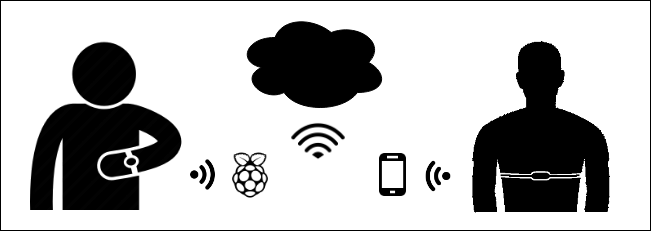
\includegraphics[width=.8\textwidth]{./img/wearable-ecosystem.png}
    \caption{\projName envisioned sensor ecosystem composed of: a wearable device, a gateway with internet connection, and the cloud were results are stored and processd.\label{fig:wearable-ecosystem}}
\end{figure}
%Both procedures lead to an approximation of R peaks' timestamps and the intervals between them (RR intervals). 
The generation of the approximated diagram (ECG or PPG) and the time measures are done inside the sensor.
Figure~\ref{fig:ecg-hrv} depicts a schematic representation of an ECG and the values streamed from the sensor to the gateway: R peak's timestamps and RR intervals. 
\begin{figure}[h!]
    \centering
    \resizebox{\linewidth}{!}{
\begin{tikzpicture}
    % Colors definition
    \pgfdeclaredecoration{single pulse}{initial}{
    \state{initial}[width=\pgfdecoratedinputsegmentlength]
    {%
        % Initial Line
        \pgfpathlineto{\pgfpoint{0.1*\pgfdecoratedinputsegmentlength}{0mm}}%    
        % P Peak
        \pgfpathsine{\pgfpoint{0.2\pgfdecorationsegmentlength}{0.15\pgfdecorationsegmentamplitude}}%
        \pgfpathcosine{\pgfpoint{0.2\pgfdecorationsegmentlength}{-0.15\pgfdecorationsegmentamplitude}}%
        % P - Q Line
        \pgfpathlineto{\pgfpoint{0.6\pgfdecorationsegmentamplitude}{0mm}}%
        % Q Valley
        \pgfpathsine{\pgfpoint{0.1\pgfdecorationsegmentlength}{-0.15\pgfdecorationsegmentamplitude}}
        \pgfpathcosine{\pgfpoint{0.01\pgfdecorationsegmentlength}{0.15\pgfdecorationsegmentamplitude}}%
        % R Peak
        \pgfpathsine{\pgfpoint{0.15\pgfdecorationsegmentlength}{\pgfdecorationsegmentamplitude}}%
        \pgfpathcosine{\pgfpoint{0.15\pgfdecorationsegmentlength}{-\pgfdecorationsegmentamplitude}}%
        % S Valley
        \pgfpathsine{\pgfpoint{0.15\pgfdecorationsegmentlength}{-0.5\pgfdecorationsegmentamplitude}}
        \pgfpathcosine{\pgfpoint{0.15\pgfdecorationsegmentlength}{0.5\pgfdecorationsegmentamplitude}}%
        % S to T line
        \pgfpathlineto{\pgfpoint{1.25\pgfdecorationsegmentamplitude}{0mm}}%
        % T Peak
        \pgfpathsine{\pgfpoint{0.8\pgfdecorationsegmentlength}{0.3\pgfdecorationsegmentamplitude}}%
        \pgfpathcosine{\pgfpoint{0.8\pgfdecorationsegmentlength}{-0.3\pgfdecorationsegmentamplitude}}%
        % Last Line
        \pgfpathlineto{\pgfpointdecoratedinputsegmentlast}%
    }
    \state{final}{}%
    }

    \fill[gray!10, draw=black] (-0.75, -0.75) rectangle (6.25, 1.75);
    \node at (-0.5, -0.5) {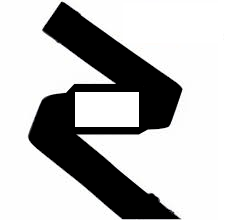
\includegraphics[width=10pt]{img/hrband.png}};
    %\node at (5.5, 1.5) {\textbf{\small{Sensor}}};

    \draw[->, dashed] (5.55,0) -- (6,0) node[pos=.5, anchor=north, xshift=-10pt] {\tiny{Time ($s$)}};
    \draw[->, dashed] (0,0) -- (0,1.25) node[anchor=south, xshift=10pt] {\tiny{Amplitude ($mV$)}};
    \draw[decoration={single pulse,amplitude=8mm,segment length=2mm},decorate] (0,0) -- (2,0);
    \draw[decoration={single pulse,amplitude=8mm,segment length=2mm},decorate] (2,0) -- (4,0);
    \draw[decoration={single pulse,amplitude=6mm,segment length=2mm},decorate] (4,0) -- (5.5,0);
    \draw[<->, dashed, thick] (0.55, 0.7) -- (2.5, 0.7);
    \draw[<->, dashed, thick] (2.55, 0.55) -- (4.35, 0.55);
    \node[align=center] at (0.5, 0.95) {\tiny{$\text{R}_0$}};
%    \node[align=center] at (2.2, 0.3) {\tiny{$\text{P}_1$}};
%    \node[align=center] at (2.45, -0.2) {\tiny{$\text{Q}_1$}};
%    \node[align=center] at (2.7, -0.55) {\tiny{$\text{S}_1$}};
%    \node[align=center] at (3.15, 0.38) {\tiny{$\text{T}_1$}};
    \node[align=center] at (2.5, 0.95) {\tiny{$\text{R}_1$}};
    \node[align=center] at (4.25, 0.8) {\tiny{$\text{R}_2$}};

    % Signal
    \fill[black] (6.5, 0) circle (0.05);
    \draw (6.75, -0.15) arc (-20:20:0.5);
    \draw (6.95, -0.25) arc (-30:30:0.5);
    \draw (7.15, -0.35) arc (-40:40:0.5);

    % Data file
    \node[align=center] at (9, 1.2) {\tiny{\textbf{\texttt{gateway://data/data\_file.csv}}}};
    \draw (7.45, -0.75) -- (7.45, 1) -- (10.5,1) -- (10.5, -0.5) to[out=180, in=0] (7.45, -0.75);
    \node[align=center] at (9, 0.2) {\tiny{\texttt{t}$\left(\text{R}_1\right)$, \xspace\texttt{t}$\left(\text{R}_1\right)$ - \texttt{t}$\left(\text{R}_0\right)$} \\ \tiny{\texttt{t}$\left(\text{R}_2\right)$, \xspace\texttt{t}$\left(\text{R}_2\right)$ - \texttt{t}$\left(\text{R}_1\right)$} \\ \tiny{\textbf{$\vdots$}}};
\end{tikzpicture}}

    \caption[Schematic representation of an ECG signal showing three normal beats.]{Schematic representation of an ECG signal showing three normal beats. A normal electrocardiogram can be broken down in three waves: a \textit{P wave} corresponding to the depolarization of the atria, a \textit{QRS complex} corresponding to the depolarization of the ventricles and a \textit{T wave} corresponding to the repolarization of the ventricle~\cite{Lilly2001}. From an ECG the sensor extracts and streams the R-peaks' timestamp and the time elapsed between them. \label{fig:ecg-hrv}}
\end{figure}

In our case, \projName focuses on the analysis of the Heart Rate Variability (HRV)~\cite{Camm1996}, that is, the analysis of the variation in the time intervals between heartbeats (a.k.a. RR intervals).
The HRV is of utmost importance since it has been shown to be a predictor for myocardial infarction~\cite{Kleiger1987,Bigger1992}.
With healthy individuals' heart rate (HR) averaging between 60 to 180 beats per minute (bpm), the average throughput per client is between 23 and 69 bytes per second.
%An interesting use case of RR processing, besides HR approximation, is the study of Heart Rate Variability (HRV). 
%HRV~\cite{hrv} is the variation in the time intervals between heartbeats and it has been proven to be a predictor of myocardial infarction.
Finally, despite \projName being specifically designed for streams with these data features, its modular design (as we later describe in Chapter \ref{chap:architecture}) makes it easy to adapt to other use-cases.

\chapter{Related Work} \label{chap:related-work}

In this Chapter we cover the related work that sets the current State-of-the-Art for privacy preserving stream processing engines of medical data.
Together with each piece of work, we provide a brief description and argue why it has or has not been considered for our project.
In \S\ref{sec:related:stream} we cover the most notable big data stream processing engines that relate with our system.
Note that stream processing is a big field and it is out of the scope of this work to provide a detailed survey.
In \S\ref{sec:related:privacy} we introduce relevant privacy-preserving processing engines: both stream and batch based.
Lastly, in \S\ref{sec:related:cardiac} we cover other approaches at cardiac data monitoring.

\section{Stream Processing Engines} \label{sec:related:stream}

Stream processing has recently attracted a lot of attention from academia and industry~\cite{Koliousis2016,Miao2017,Venkataraman2017}.
Apache Spark~\cite{Zaharia2012} is arguably the de-facto standard in this domain, by combining batch and stream processing with a unified API~\cite{ZahariaDStreams2012}.
Apache Spark SQL~\cite{Armbrust2015} allows to process structured data by integrating relational processing with Spark's functional programming style.
Structured streaming~\cite{Armbrust2018} leverages Spark SQL and it compares favorably against the discretized counterpart~\cite{ZahariaDStreams2012} in terms of performance. % approach used in this project. 
However, the former lacks security or privacy guarantees, and hence it was not considered.
Furthermore \sgxspark only has support for the \textit{Discretized Streams} API, and therefore we also rely on it.

\section{Privacy-Preserving Computation} \label{sec:related:privacy}

Opaque~\cite{Zheng2017} is a privacy-preserving distributed analytics system.
It leverages Spark SQL and Intel SGX enclaves to perform computations over encrypted Spark DataFrames.
In \texttt{encryption} mode, Opaque offers security guarantees similar to our system's.
However, \emph{(1)} the Spark master must be located in the client side, for it must be trusted. 
An scenario that does not fit in our multi-client setting.
And \emph{(2)}, it requires changes to the application code, and hence is not transparent to the user.
In \texttt{oblivious} mode, \emph{i.e.}, protecting against traffic pattern analysis attacks, it can be up to $46\times$ slower, a slow-down factor not tolerable for the real-time analytics in the scope of our system.

SecureStreams~\cite{Havet2017} is a reactive framework that exploits Intel SGX to define dataflow processing by pipelining several independent components. 
In order to use this framework, the user requires a good knowledge of the underlying implementation. 
Moreover, applications must be written in the \textsc{Lua} programming language, hindering its applicability to legacy systems or third-party programs.

\textsc{DPBSV}~\cite{Puthal2015} is a secure big data stream processing framework that focuses on securing data transmission from the sensors or clients to the \textit{Data Stream Manager (DSM)} or server. 
Its security model requires a \textit{Public Key Infrastructure (PKI)} and a dynamic prime number generation technique to synchronously update the keys. 
In spite of using trusted hardware on the DSM end for key generation and management, the server-side processes all the data in clear, making the framework not suitable for our security model. 

\textsc{TaLoS}~\cite{Aublin2017} is a \textit{Transport Layer Security (TLS)}~\cite{Dierks2008} library that terminates connections by maintaining sensitive information inside enclaves. 
The authors provide custom wrappers for the most common \textsc{TLS} API calls and securely store users and sessions' keys inside enclaves.
The embedding with a native Spark, or SGX-Spark, application is not transparent to the end user and hence why we discard it.

Lastly, homomorphic encryption~\cite{Gentry2009} does not rely on trusted execution environments and offers the promise of providing privacy-preserving computations over encrypted data.
This is, it generates an encrypted result from two encrypted operands, corresponding to the encrypted value of operating both operands in plain text.
The key feature of the scheme is that, at no point, neither the operands nor the result are processed in clear.
While several works analyzed the feasibility of homomorphic encryption schemes in cloud environments~\cite{Tetali2013,Stephen2016}, the performance of homomorphic operations~\cite{Gottel2018} is far from being pragmatic.

\section{Cardiac Monitoring Systems} \label{sec:related:cardiac}
% \vs{briefly discuss \cite{Puthal:2015:DES:2847604.2848495}}
% Talk about medical things
For the specific problem of HRV analysis, while periodic monitoring solutions exist~\cite{Renevey2018}, they are focused on embedded systems.
As such, since they off-load computation to third-party cloud services, these solutions simply overlook the privacy concerns that we consider.
Similarly, another solution~\cite{VanZaen2019} uses convolutional networks for the detection of arrhythmias.
However, the authors take no considerations with regard to data security and privacy.

%To the best of our knowledge, there are no privacy-preserving real-time streaming systems specifically designed for  medical and cardiac data. 
This work is one of the first attempts to building a privacy-preserving real-time streaming system specifically designed for  medical and cardiac data. 

Our system fills the existing research gap by proposing a system that leverages Intel SGX enclaves to compute such analytics over public untrusted clouds without changing the existing Scala-based source code.
 % TODO: think wether I merge this section into BG
\chapter{Architecture} \label{chap:architecture}

The aim of this Chapter is to depict \projName's architecture.
A high-level abstraction is presented in Figure~\ref{fig:system-architecture}, where each different component is represented together with the path data follows.
\projName has a client-server organization and each functionality is designed to be modular and self-contained for the ease of deployment, evaluation, scalability and availability.
On general lines, the server-side component is executed on untrusted machines (for instance nodes on the cloud) where Intel SGX is vailable.
On the remote end, the \sgxspark engine is deployed and stream processes the data generated by an arbitrary number of clients.
Each client is a sensor generating samples, and a gateway aggregating them and sending them periodically to the cloud-based component.
Similarly, clients fetch the results at fixed time intervals.
The interaction between the clients and the server happens over a filesystem interface hosted at the server-side.
Each client data stream is processed in parallel by the processing engine independently of the chosen algorithm.

The remaining of the chapter is structured as follows: \S\ref{sec:server} details the server-side architecture, \S\ref{sec:client} does the same with the client-side component, in \S\ref{sec:threat} we cover the considered threat model and the security assumptions we make in the design and lastly in \S\ref{sec:vulnerabilities} we present \projName's known vulnerabilities.

\begin{figure}[h!]
    \centering
    \resizebox{\linewidth}{!}{
\begin{tikzpicture}
    % Colors definition: latexcolor.com
    \definecolor{ashgrey}{rgb}{0.7, 0.75, 0.71}
    \definecolor{x11gray}{rgb}{0.75, 0.75, 0.75}
    \definecolor{metal}{rgb}{0.43, 0.5, 0.5}

    
    % Main outline
    % Background
    \draw[fill=gray!10] (0, 2.75) rectangle (6.75, 6.0);

    % Client Side
    % Client boxes line
    % Client 1
    \draw[fill=gray!5] (0,1.5) rectangle (2, 2.25);
    \node at (1.6, 1.825) {
\includegraphics[width=10pt]{img/smartwatch.png}};
    \node at (1.05, 1.825) {
\includegraphics[width=10pt]{img/wifi-signal.png}};
    \node at (0.4, 1.825) {
\includegraphics[width=15pt]{img/raspberry.png}};
    % Client 2
    \draw[fill=gray!5] (2.5,1.5) rectangle (4.5, 2.25);
    \node at (2.9, 1.825) {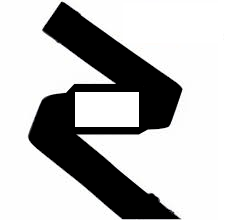
\includegraphics[width=10pt]{img/hrband.png}};
    \node at (3.5, 1.825) {
\includegraphics[width=10pt]{img/wifi-right.png}};
    \node at (4.1, 1.825) {
\includegraphics[width=15pt]{img/raspberry.png}};
    % Client 3
    \node at (5.265, 1.85) {$\cdots$};
    \draw[fill=gray!5] (5.85,1.5) rectangle (6.9, 2.25) node[pos=.5] {\tiny{Client $m$}};
    \draw[fill=gray!5] (8.875,1.5) rectangle (9.625, 2.25) node[pos=.5] {\tiny{Client}};
    % Lines to filesystem
    \draw[<->, dashed, thick] (0.4, 2.25) -- (0.4, 3.5) -- (1, 3.5);
    \draw[<->, dashed, thick] (4.1, 2.25) -- (4.1, 2.35) -- (1.35, 2.35) -- (1.35, 3);
    \draw[<->, dashed, thick] (6.3725, 2.25) -- (6.3725, 2.55) -- (1.85, 2.55) -- (1.85, 3);
    \draw[dashed, thin] (8.875, 2.25) -- (8, 2.75);
    \draw[dashed, thin] (9.625, 2.25) -- (10.5, 2.75);

    % Server Side
    % FileSystem Logo
    \draw[fill=x11gray!50] (1.0, 3) -- (1.1, 3.9) -- (1.6, 3.9) -- (1.75, 4.0) -- (2.1, 4.0) -- (2.0, 3);
    %\draw[fill=x11gray] (1.0, 3) -- (1.0, 3.8) -- (1.6, 3.8) -- (1.75, 3.6) -- (2.0, 3.6) -- (2.0, 3) -- (1.0, 3);
    \node[align=center] at (1.4, 5.1) {\text{\tiny{\textbf{FileSystem}}} \\[-8pt] \text{\tiny{\textbf{Interface}}}};
    % SGX Spark
    % Main Outline
    \draw[fill=white] (2.75, 3) rectangle (6.25, 5.5);
    \node at (4.4, 5.7) {\text{\textbf{\tiny{SGX-Spark Engine}}}};
    % SHM
    \draw (2.95, 3.2) rectangle (6.05, 3.5) node[pos=.5] {\tiny{Host Shared Memory}};
    % Driver
    \draw[pattern=north west lines,pattern color=gray!50] (2.95, 3.7) rectangle (3.95, 4.4); 
    \node at (3.75, 4.5) {\tiny{\texttt{driver-enclave.sh}}};
    \node at (2.95, 3.7) {
\includegraphics[width=8pt]{img/intel-sgx.png}};
    \draw (2.95, 4.6) rectangle (3.95, 5.3); 
    \node at (3.35, 5.4) {\tiny{\texttt{driver.sh}}};
    % Worker
    \draw[pattern=north west lines,pattern color=gray!50] (4.15, 3.7) rectangle (6.05, 4.4);
    \node at (4.9, 3.6) {\tiny{\texttt{worker-enclave.sh}}};
    \draw (4.15, 4.6) rectangle (6.05, 5.3);
    \node at (5.55, 5.4) {\tiny{\texttt{worker.sh}}};
    % Tasks Enclave
    \draw[fill=white] (4.25, 3.8) rectangle (4.65, 4.3) node[pos=.5] {\tiny{$T_1$}};
    \draw[fill=white] (4.75, 3.8) rectangle (5.15, 4.3) node[pos=.5] {\tiny{$T_2$}};
    \node at (5.35, 4.05) {\tiny{$\cdots$}};
    \draw[fill=white] (5.55, 3.8) rectangle (5.95, 4.3) node[pos=.5] {\tiny{$T_N$}};
    \node at (6, 3.7) {
\includegraphics[width=8pt]{img/intel-sgx.png}};
    % Tasks Outside Enclave
    \draw (4.25, 4.7) rectangle (4.65, 5.2) node[pos=.5] {\tiny{$T_1$}};
    \draw (4.75, 4.7) rectangle (5.15, 5.2) node[pos=.5] {\tiny{$T_2$}};
    \node at (5.35, 4.95) {\tiny{$\cdots$}};
    \draw (5.55, 4.7) rectangle (5.95, 5.2) node[pos=.5] {\tiny{$T_N$}};

    % CSEM's Toolbox
    \draw[fill=white] (0.8, 3.7) rectangle (2.1, 4.75);
    \node at (1.45, 4.55) {\textsc{\tiny{CSEM HRV}}};
    \draw[dashed] (0.8, 4.4) -- (2.1, 4.4);
    \node[align=left] at (1.42, 4.25) {\texttt{\tiny{+ Identity}}};
    \node[align=left] at (1.19, 4.05) {\texttt{\tiny{+ SDNN}}};
    \node[align=left] at (1.42, 3.85) {\texttt{\tiny{+ HRVBands}}};
    \draw[fill=x11gray] (1.0, 3) -- (1.0, 3.8) -- (1.6, 3.8) -- (1.75, 3.6) -- (2.0, 3.6) -- (2.0, 3) -- (1.0, 3);

    % Client Expansion
    % Separator
    \draw (7.3, 1.5) -- (7.3, 6);
    \draw (7.5, 1.5) -- (7.5, 6);
    % Client itself
    \draw[fill=gray!10] (8, 2.75) rectangle (10.5, 5.55);
    %\draw (9.25, 1.3725) circle (0.5);
    \draw[dashed] (8, 3.55) -- (10.5, 3.55);
    \draw[fill=white] (8.2, 2.95) rectangle (10.3, 3.35) node[pos=.5] {\tiny{\texttt{sensor}}};
    \node at (10.3, 3.00) {
\includegraphics[width=10pt]{img/docker.png}};
    \node at (8.2, 3.00) {
\includegraphics[width=8pt]{img/smartwatch.png}};
    \draw[fill=white] (8.2, 3.75) rectangle (10.3, 4.15) node[pos=.5] {\tiny{\texttt{eclipse-mqtt}}};
    \node at (10.3, 3.80) {
\includegraphics[width=10pt]{img/docker.png}};
    \draw[fill=white] (8.2, 4.35) rectangle (10.3, 4.75) node[pos=.5] {\tiny{\texttt{mqtt-subscriber}}};
    \node at (10.3, 4.40) {
\includegraphics[width=10pt]{img/docker.png}};
    \draw[fill=white] (8.2, 4.95) rectangle (9.2, 5.35) node[pos=.5] {\tiny{\texttt{consumer}}};
    \node at (8.3, 5.00) {
\includegraphics[width=10pt]{img/docker.png}};
    \draw[fill=white] (9.3, 4.95) rectangle (10.3, 5.35) node[pos=.5] {\tiny{\texttt{producer}}};
    \node at (10.3, 5.00) {
\includegraphics[width=10pt]{img/docker.png}};
    \draw[->, very thick, dashed] (9.8, 5.35) -- (9.8, 6);
    \draw[<-, very thick, dashed] (8.7, 5.35) -- (8.7, 6);

\end{tikzpicture}}

    \caption{(Left) Schematic of the system's main architecture. A set of clients bidirectionally stream data to a remote server. The interaction is done via a filesystem interface. On the server side, \sgxspark performs secure processing using different HRV analysis algorithms. (Right) Breakdown of a packaged client: it includes a \texttt{sensor} and gateway that wrap four different microservices (\textsc{mqtt} broker, \texttt{mqtt-subscriber}, \texttt{consumer}, \texttt{producer}) to interact with the remote end. \label{fig:system-architecture}}
\end{figure}

\section{Server-Side} \label{sec:server}

The server-side component is made by three different modules: a filesystem interface, the \sgxspark engine, and a set of algorithms to analyze HRV. 
The filesystem interface acts as a landing point for the batches of data generated by each client. 
It is monitored by the \sgxspark engine.
Currently, it is mounted and unmounted, respectively at start-up time and upon the shutdown of the service. 
The streaming engine and the pool of algorithms are compiled together by the same toolchain, yet they are independent. 
The \textsc{Spark} engine (deployed in standalone mode) executes: the master process, the driver process, and an arbitrary number of workers. 
In the case of \sgxspark jobs, two JVMs are deployed per driver and worker process: one inside an enclave and one outside.
The communication between JVMs is kept encrypted and is done through the host OS shared memory (see Figure \ref{fig:sgx-spark-scheme}).
%the driver and the worker run in separated JVMs, isolated from each other.
%These JVMs are \emph{duplicated}, in the sense that the driver and each worker .
%Each JVM is, at the same time, duplicated\vs{what do you mean?}, with its counterpart running inside an enclave.
For each JVM pair, \sgxspark will initialize a new enclave.
% Being one located inside the enclave and another one outside. 
The specific algorithm that \projName will execute is currently set at start-up time, although several concurrent ones can be executed, each yielding separated results. 

\section{Clients} \label{sec:clients}

The client is a combination of: (1) a data generator that simulates a sensor and (2) a gateway that interacts with the remote end. 
The data generator streams RR intervals. %synthetic 
These samples are gathered by the gateway, which stacks and sends them for processing in a file-based streaming fashion. 
The typical size of these batches is in the 230---690 Bytes range.
Each gateway is composed by: a message broker that handles the samples, a service that handles data pre-processing and batch sending, and a fetcher that directly greps from the server's filesystem.

\section{Threat Model} \label{sec:threat}

We assume that the communication between the gateway and the filesystem is kept protected (\emph{e.g.}, encrypted) using secure transfer protocols (more in Section~\ref{sec:implementation}).
Given this assumption, \projName's threat model is the same as typical systems that rely on \textsc{SGX}. 
Specifically, we assume the system software is  untrusted.
Our security perimeter only includes the internals of the CPU package. 
The trusted computing base is Intel's microcode as well as and the code loaded at the enclave, which can be measured and integrity checked. 
In \projName, we assume that the client package is trusted and tamper-proof.
We focus on protecting the areas \emph{outside} user's control. 
However, if the client package is deployed in, for instance, a \textsc{Raspberry Pi}, the TCB could be further reduced using .

\section{Known Vulnerabilities} \label{sec:vulnerabilities}

As for the known vulnerabilities, \textsc{SGX} (in particular the memory encryption engine) is not designed to be an oblivious RAM.
As a consequence and adversary can perform traffic analysis attacks~\cite{Gueron2016}.
Moreover, side-channel attacks~\cite{sgx-sidechannel} and speculative execution attacks (\textit{Spectre}-like~\cite{sgx-spectre} and \textit{Foreshadow}~\cite{foreshadow}) have still successful against enclaves and will require in-silicon fixes.

\chapter{Implementation} \label{chap:implementation}
% TODO: include code listings in this section!!
% TODO: Add appendix with all docker deployment files.

The aim of this chapter is to present the implementation details of \projName.
Each explanation is accompanied, when required, by code snippets to further illustrate the rationale behind our design choices.
The implementation we will cover is the one the results presented in Chapter \ref{chap:evaluation} are based on.
As a consequence, and in order to stress-test \projName, we replace real sensors with synthetic data generators.
Additionally, all components are packaged in Docker containers so that a large fleet of clients concurrently using our system can be replicated.
In \S\ref{sec:server-implementation} and \S\ref{sec:client-implementation} we cover the implementation details of the server-side and the client-side component respectively.
Re-using Docker-speciphic nomenclature, we will there refer to functionalities packaged in a container as services.
A collection of services makes up one component.
Lastly, in \S\ref{sec:deployment} we cover how we establish the client cluster and deploy hundreds of fake users.
Furthermore, in Appendix REF, we attach all the Docker configuration scripts together with the main source code. %TODO: appendix!!

\section{Server Implementation} \label{sec:server-implementation}

\section{Client Implementation} \label{sec:client-implementation}

\section{Deployment} \label{sec:deployment}

\section{Evaluation} \label{sec:evaluation}

\chapter{Future Work} \label{chap:future-work}

\chapter{Conclusions and Lessons Learnt} \label{chap:conclusion}


% Bibliography: for the different bibliography styles see https://www.overleaf.com/learn/latex/Bibtex_bibliography_styles
%\pagebreak
\bibliographystyle{unsrt}
\bibliography{references}

\begin{appendices}
    \chapter{Implementation Code Snippets} \label{chap:app-code}

\section{Server-Side Algorithms}

\begin{lstlisting}[language=Scala,caption={Implementation of the \texttt{SDNN} algorithm.},label=code:sdnn]
/** Estimation of the Standard Deviation between NN intervals.
 *                                                                
 *  @constructor create a new estimation suite.
 *  @param wdwSize duration in seconds of the window in which we compute
 *  the standard deviation.
 */                                                                   
class EstimateSDNN(wdwSize: Int) { 

  /** Estimation of the SDNN with a fixed window in streaming mode
   *
   *  @return returns a DStream containing a tuple per line containing the time
   *  block/interval (starting from zero) and the SDNN value.
   */
  def sdnn(dataStream: DStream[String]): DStream[(String, Double)] = {
    val operatorByKey = new StreamOperators(wdwSize)
    operatorByKey.sumSquareByKey(dataStream)
      .join(operatorByKey.cardinalByKey(dataStream))
      .map(udfDivide)
      .join(operatorByKey.avgByKey(dataStream))
      .map(udfSqrtDif)
      .map(udfTimesWindow)
  }

}
\end{lstlisting}

\begin{lstlisting}[language=Scala,caption={Implementation of the \texttt{HRVBands} algorithm.},label=code:hrvbands]
package org.apache.spark.csem.utils

import org.apache.spark.rdd.RDD
import org.apache.spark.streaming.dstream.DStream
import org.apache.spark.csem.utils.StreamOperators

import scala.math.{pow, cos, sin, Pi, floor}

/** Set of signal processing operators defined on (K, V), (String, Float) 
 *  DStreams. Currently the methods included in this suite are: DFT,
 *
 *  @constructor create a new operator suite. 
 *  @param wdwSize duration in seconds of the window in which we compute
 *  the standard deviation.
 */
class StreamSignalProcessing(wdwSize: Int) extends Serializable {

  /** Preprocesses the input data stream (which contains lines from the csv
   *  input file) to the following format, (k, v) where:
   *  - k: is the 10 second block identifier (key)
   *  - v: iterable with all the rr's from that block indexed.
   *
   *  @return A data stream with the specified format.
   */
  def preProcess(dataStream: DStream[String]):
    DStream[(String, Iterable[(Double, Int)], Int)] = {
      dataStream
        .map(line => (floor(line.split(",")(0).toDouble/10).toInt.toString,
          line.split(",")(1).toDouble))
        .groupByKey()
        .map(line => (line._1, line._2.zipWithIndex, line._2.size))
  }

  /** Compute the squared module of the Discrete Fourier Transform of the 
   *  samples contained in the DStream.
   *
   *  @return returns a DStream containing a tuple per line containing the time
   *  block/interval (starting from zero) and the sum of all the values
   *  in that same interval.
   */
  def modDFT2(dataStream: DStream[String]):
    DStream[(String, Double, Double, Double)] = { 

    // Auxiliary methods to compute the squared modulus of the DFT
    def cosDFT(line: (String, Iterable[(Double, Int)], Int), f_index: Int):
      Double = {
      line._2
        .map(x => x._1*cos(2*Pi*x._2*f_index/line._3))
        .reduce((a,b) => (a+b))
    }
    def sinDFT(line: (String, Iterable[(Double, Int)], Int), f_index: Int):
      Double = {
      line._2
        .map(x => x._1*sin(2*Pi*x._2*f_index/line._3))
        .reduce((a,b) => (a+b))
    }

    // Compute the Square Modulus of the DFT
    def modDFT(value: (Double, Int),
      line: (String, Iterable[(Double, Int)], Int)): (Double, Int) = {
        (pow(cosDFT(line, value._2), 2) + pow(sinDFT(line, value._2), 2),
          value._2)
    }

    // Predicate to know if a value belongs to the High Freq. Component
    def isHighFreq(value: (Double, Int), cardinal: Int): Boolean = {
      val thr_low = (0.15 * cardinal).toInt
      val thr_high = (0.4 * cardinal).toInt
      value._2 match {
        case x if thr_low until thr_high contains x => true
        case _ => false
      }
    }

    // Predicate to know if a value belongs to the Low Freq. Component
    def isLowFreq(value: (Double, Int), cardinal: Int): Boolean = {
      val thr_low = (0.04 * cardinal).toInt
      val thr_high = (0.15 * cardinal).toInt
      value._2 match {
        case x if thr_low until thr_high contains x => true
        case _ => false
      }
    }

    val tmp = preProcess(dataStream)
      .map( l => (l._1, l._2.map( list => modDFT(list, l) ), l._3) )

    // High Frequency Component
    val highFreq = tmp
      .map(line => (line._1, line._2
        .filter( x => isHighFreq(x, line._3) )
        .map( x => x._1 )
        .foldLeft(0.toDouble)( (a,b) => (a + b) ), line._3))
      .map( line => (line._1, line._2 / pow(line._3, 2) * 2) )

    // Low Frequency Component
    val lowFreq = tmp
      .map(line => (line._1, line._2
        .filter(x => isLowFreq(x, line._3))
        .map( x => x._1 )
        .foldLeft(0.toDouble)( (a,b) => (a + b) ), line._3))
      .map( line => (line._1, line._2 / pow(line._3, 2) * 2) )
    lowFreq
      .join(highFreq)
      .map( x => (x._1, x._2._1, x._2._2, x._2._1 / x._2._2) )
  }
}


/** Estimation of the frequency bands given a HRV sequence.
 *
 *  @constructor create a new estimation suite.
 *  @param wdwSize duration in seconds of the window in which we estimate
 *  the frequency bands.
 */
class EstimateHRVBands(wdwSize: Int) {
  /** Estimation of the SDNN with a fixed window in streaming mode
   *
   *  @return returns a DStream containing a tuple per line containing the time
   *  block/interval (starting from zero) and the SDNN value.
   */
  def estimate(dataStream: DStream[String]):
      DStream[(String, Double, Double, Double)] = {
    val processingByKey = new StreamSignalProcessing(wdwSize)
    processingByKey.modDFT2(dataStream)
  }
}
\end{lstlisting}

\begin{lstlisting}[language=Scala,caption={Implementation of the \texttt{Identity} algorithm.},label=code:identity]
/** Main application/class that launches the identity application.                                                [64/180]
 *                                                                                                                        
 *  @note We implement the identity application that                                                 
 *  basically does nothing. This way we will be able to measure easily the                                                
 *  system's overhead.
 */
object Identity extends Logging {

  def main(args: Array[String]) {

    // Initialize Variables and Spark Context
    val numClients = args(0).toInt
    val conf = new SparkConf().setAppName("HRV Toolbox - Identity")
    val sc = new SparkContext(conf)
    val ssc = new StreamingContext(sc, Duration(10000))

    // Map Output to Input
    val dataStreamVec = for (i <- 1 to numClients) yield ssc.textFileStream("csem/src/main/resources/csv/"+i.toString+"/
")
    for (i <- 1 to numClients) {
    dataStreamVec(i-1).saveAsTextFiles("csem/src/main/resources/results/" + i.toString + "/identity")
    }

    ssc.start()
    ssc.awaitTermination()
  }
}
\end{lstlisting}

\section{Client-Side Services Source Code}

\begin{lstlisting}[language=Python,caption={Implementation of the \texttt{sensor} service.},label=code:sensor]
"""Fake MQTT Generator

This module emulates a sensor that publishes data to a MQTT topic with a given
sample rate.
"""
// Method names are those required to be overridden by Paho MQTT
import paho.mqtt.publish as publish 
import signal
import sys
import time
from datetime import datetime
from numpy import random


// SIGTERM Signal Handler
class Killer:
  kill_now = False
  def __init__(self):
    signal.signal(signal.SIGTERM, self.exit_gracefully)

  def exit_gracefully(self, signum, frame):
    self.kill_now = True

    
// Callback to be executed at service start up time
def run(sample_rate):
    if sample_rate == 0:
        raise ZeroDivisionError("Can not set a 0 sample rate")
    loop(int(sample_rate))


def loop(sample_rate):
    """Endless Sample Generation

    This module is the endless loop that generates <sample_rate>
    new samples per second and publishes them to a MQTT topic.

    Parameters
    ----------
    sample_rate : float
        How many samples are generated per second
    """
    killer = Killer()
    global CL_ID
    past_ts = time.time()
    while 1:
        value = ""
        # First we generate <sample_rate> timestamps in one second
        tstamps = [i for i in random.uniform(low=time.time(),
                                             high=time.time() + 1,
                                             size=(sample_rate))]
        tstamps.sort()
        # Second we compute the intervals between them
        for i in tstamps:
            tmp = datetime.fromtimestamp(i).strftime('%Y-%m-%d %H:%M:%S')
            value += tmp+','+str(int((i - past_ts) * 1e6))+'\n'
            past_ts = i
        publish.single("artificial-data-{}".format(CL_ID), value)
        time.sleep(1)
        if killer.kill_now:
            print("Exitting gracefully!")
            break


if __name__ == "__main__":
    """Standalone entry point"""
    if len(sys.argv) < 2:
        raise TypeError("No Sample Rate provided")
    CL_ID = sys.argv[2]
    run(sys.argv[1])
\end{lstlisting}

\begin{lstlisting}[language=Python,caption={Implementation of the \texttt{mqtt-subscriber} service.},label=code:mqtt-sub]
"""MQTT Subscriber and CSV Generator

This module subscribes to the data topic in a MQTT queue and, whenever it
stacks a given amount of samples it generates a new csv file.

Attributes
----------
count : int
    Global counter.
curr_str : str
    Global string accumulator.
"""
import paho.mqtt.client as mqtt
from datetime import datetime
import time
import signal
import sys
import os


count = 0
curr_str = ""


class Killer:
  kill_now = False
  def __init__(self):
    signal.signal(signal.SIGTERM, self.exit_gracefully)

  def exit_gracefully(self, signum, frame):
    self.kill_now = True


def on_message(mosq, obj, msg):
    """Callback method for the mosquitto client.

    Whenever the MQTT client receives a new sample it triggers this method.
    When the current count reaches the threshold, a new csv file is generated
    and stored in the local data directory.

    Parameters
    ----------
    Parameters are those of the standard implementation of the MQTT client
    for Python.
    """
    global count
    global curr_str
    global FILE_LINES
    global CL_ID
    global LOCAL_DATA_DIR
    global killer
    print("Received message")
    dcd_msg = msg.payload.decode("utf-8").split("\n")
    whole_msg = [i.split(",") for i in dcd_msg if i != ""] 
    for tmp in whole_msg:
        d = datetime.strptime(tmp[0], '%Y-%m-%d %H:%M:%S')
        time_stamp = time.mktime(d.timetuple())
        rr = tmp[1]
        if count == FILE_LINES:
            global TS
            print("It took: {} s".format(time.time() - TS))
            curr_str += "{},{}".format(time_stamp, rr)
            ts = int(time.time()*1e3)
            filename = "{}{}_".format(LOCAL_DATA_DIR, CL_ID)+str(ts)+".csv"
            try:
                with open(filename, "w+") as f:
                    f.write(curr_str)
            except FileNotFoundError as e:
                if killer.kill_now:
                    mosq.disconnect()
                    print("Exitting gracefully!")
                    break
            count = 0
            curr_str = ""
        else:
            curr_str += "{},{}\n".format(time_stamp, rr)
            count += 1
    else:
        if killer.kill_now:
            mosq.disconnect()
            print("Exitting gracefully!")


def start_mqtt():
    """Start the MQTT client"""
    global CL_ID
    mqttc = mqtt.Client()
    mqttc.on_message = on_message
    mqttc.connect("localhost", port=1883)
    mqttc.subscribe("artificial-data-{}".format(CL_ID))
    mqttc.loop_forever()


if __name__ == "__main__":
    """Standalone execution entry point"""
    try:
        FILE_LINES = int(sys.argv[1])
    except IndexError as e:
        print("Have not provided a FILE_LINES value!")
        sys.exit(1)
    killer = Killer()
    CL_ID = sys.argv[2]
    LOCAL_DATA_DIR = sys.argv[3]
    start_mqtt()
    TS = time.time()
\end{lstlisting}

\begin{lstlisting}[language=Python,caption={Implementation of the \texttt{producer} service.},label=code:producer]
"""CSV Producer

This module monitors a local data directory and perodically sends the newly
added csv files to a remote directory in order to be processed.

Attributes
----------
"""
import os
import time
import signal
import sys
from paramiko import SSHClient, SSHConfig, ProxyCommand, SFTPClient
from paramiko.util import log_to_file
from server_connect import server_connect


class Killer:
  kill_now = False
  def __init__(self):
    signal.signal(signal.SIGTERM, self.exit_gracefully)

  def exit_gracefully(self, signum, frame):
    self.kill_now = True


def monitor(ssh, sftp, *args):
    """Sending daemon

    This method starts an infinite loop that every <SEND_PERIOD> looks for
    newly added data files and copies them to a remote directory.

    Parameters
    ----------
    ssh : paramiko.SSHClient
        SSH Client connected to the remote host.
    sftp : paramiko.SFTPClient
        SFTP Client connected to the remote host.
    """
    global LOCAL_DATA_DIR
    path_to_watch = LOCAL_DATA_DIR
    before = dict([(f, None) for f in os.listdir(path_to_watch)])
    global SEND_PERIOD
    killer = Killer()
    while 1:
        time.sleep(SEND_PERIOD)
        after = dict([(f, None) for f in os.listdir(path_to_watch)])
        added = [f for f in after if f not in before]
        if added:
            for f in added:
                local_file = LOCAL_DATA_DIR + str(f)
                global REMOTE_DATA_DIR
                remote_file = REMOTE_DATA_DIR + "/" + str(f)
                sftp.put(local_file, remote_file)
                os.remove(local_file)
                # If there are a lot of files, not checking inside also leads
                # to error with code 137
                if killer.kill_now:
                    print("Exitting gracefully!")
                    break
        before = after
        if killer.kill_now:
            print("Exitting gracefully!")
            break
    for d in os.listdir(LOCAL_DATA_DIR):
        tmp_file = LOCAL_DATA_DIR + str(d)
        os.remove(tmp_file)


if __name__ == "__main__":
    """Standalone entry point

    The scripts is executed as a subprocess and as a consequence in standalone
    mode. This is done to prevent it from blocking the rest of the execution
    and to prevent from working with Python's threading library.
    """
    ssh, sftp = server_connect()
    LOCAL_DATA_DIR = sys.argv[1]
    REMOTE_DATA_DIR = sys.argv[2]
    SEND_PERIOD = int(sys.argv[3])
    sftp.mkdir(REMOTE_DATA_DIR)
    monitor(ssh, sftp)
\end{lstlisting}

\begin{lstlisting}[language=Python,caption={Implementation of the \texttt{consumer} service.},label=code:consumer]
"""Result Consumer Daemon

This module periodically fetches data from a remote directory containing the
results of the computation and copies them over SFTP to a local directory.

Attributes
----------
FETCH_PERIOD : int
    How often does the module fetch the newly generated directories.
"""
import os
import getpass
import sys
import time
import signal
from paramiko import SSHClient, SSHConfig, ProxyCommand, SFTPClient
from paramiko.util import log_to_file
from server_connect import server_connect


class Killer:
  kill_now = False
  def __init__(self):
    signal.signal(signal.SIGTERM, self.exit_gracefully)

  def exit_gracefully(self, signum, frame):
    self.kill_now = True


def get_all(sftp, remote_dir, local_dir):
    """Copy a whole directory

    The aim of this module is to emulate the -r option in scp. Note that this
    is not recursive and only works in a folder with a known and given
    structure.

    Parameters
    ----------
    sftp : paramiko.SFTPClient
        SFTP Client connected to the remote host.
    remote_dir : str
        Path of the directory we are copying from.
    local_dir : str
        Path of the directory we are copying to.
    """
    for f in sftp.listdir(remote_dir):
        remote_file = remote_dir + str(f)
        if (not f.startswith('.')) and (not f.startswith('_')):
            local_file = local_dir + str(f)
            sftp.get(remote_file, local_file)


def monitor(ssh, sftp):
    """Fetching daemon

    This method starts an infinite loop that every <FETCH_PERIOD> looks for
    newly added directories and copies them to a local result directory.

    Parameters
    ----------
    ssh : paramiko.SSHClient
        SSH Client connected to the remote host.
    sftp : paramiko.SFTPClient
        SFTP Client connected to the remote host.
    """
    global REMOTE_RESULT_DIR
    global FETCH_PERIOD
    global LOCAL_RESULT_DIR
    #print("CONSUMER: user -> {}".format(getpass.getuser()))
    path_to_watch = REMOTE_RESULT_DIR
    before = dict([(f, None) for f in sftp.listdir(path_to_watch)])
    killer = Killer()
    while 1:
        time.sleep(FETCH_PERIOD)
        after = dict([(f, None) for f in sftp.listdir(path_to_watch)])
        added = [f for f in after if f not in before]
        if added:
            for f in added:
                local_dir = LOCAL_RESULT_DIR + str(f) + "/"
                remote_dir = REMOTE_RESULT_DIR + "/" + str(f) + "/"
                try:
                    os.mkdir(local_dir)
                    get_all(sftp, remote_dir, local_dir)
                except FileExistsError as e:
                    print("Fetching a file that already exists!")
        before = after
        if killer.kill_now:
            print("Exitting gracefully!")
            break
    for d in os.listdir(LOCAL_RESULT_DIR):
        tmp_dir = LOCAL_RESULT_DIR + d
        for f in os.listdir(tmp_dir):
            tmp_file = tmp_dir + "/" + f
            os.remove(tmp_file)
        os.rmdir(tmp_dir)


if __name__ == "__main__":
    """Standalone entry point

    The scripts is executed as a subprocess and as a consequence in standalone
    mode. This is done to prevent it from blocking the rest of the execution
    and to prevent myself from working with Python's threading library.
    """
    ssh, sftp = server_connect()
    LOCAL_RESULT_DIR = sys.argv[1]
    REMOTE_RESULT_DIR = sys.argv[2]
    sftp.mkdir(REMOTE_RESULT_DIR)
    FETCH_PERIOD = int(sys.argv[3])
    monitor(ssh, sftp)
\end{lstlisting}
\section{Deployment Scripts}

\begin{lstlisting}[language=Python,caption={Server-Side Deployment Script.},label=code:deployment:server]
#!/usr/bin/python3
"""Remote Side Standalone MedSpark Launcher

This module implements the remote-side, standalone, launcher for MedSpark.
"""
import os
import sys
import time
import signal
from server_connect import server_connect


class Killer:
  kill_now = False
  def __init__(self):
    signal.signal(signal.SIGTERM, self.exit_gracefully)

  def exit_gracefully(self, signum, frame):
    self.kill_now = True


def main(ssh, sftp):
    """Main execution method

    This method contains the main deployment of UC1. It basically starts each
    and every process, launches the benchmarking, and cleans everything when
    execution has finished.

    Notes
    -----
    All the sleeps are placed due to experienced errors race conditions. As a
    consequence their arguments are completely empirical.

    Arguments
    ---------
    ssh : paramiko.SSHClient
        SSH Client to the remote server.
    sftp : paramiko.SFTPClient
        SFTP Client to the remote server.
    """
    global ALGORITHM
    global SGX_MODE
    global NUM_CLIENTS
    algo_name = "./launch-csem-{}.sh {}".format(ALGORITHM, NUM_CLIENTS)
    if SGX_MODE:
        script_list = ["./master.sh", "./worker.sh", "./worker-enclave.sh",
                       "./driver-enclave.sh", algo_name]
    else:
        script_list = ["./master.sh", "./worker.sh", algo_name]
    for script in script_list:
        _in, _out, _err = ssh.exec_command("cd sgx-spark; {} &".format(script))
        time.sleep(3)
    tmp_command = "dstat -l --nocolor --noheaders 10 > cpu_load.csv"
    _, _out, __ = ssh.exec_command("cd sgx-spark; {} &".format(tmp_command))
    _out.readlines()
    killer = Killer()
    while 1:
        time.sleep(1)
        if killer.kill_now:
            print("Killing Gracefully!")
            break
    for script in script_list:
        _, _out, __ = ssh.exec_command("kill $(pgrep -f '{}')".format(script))
        _out.readlines()
    _, _out, __ = ssh.exec_command("kill $(pgrep -f 'java')")
    _out.readlines()
    _, _out, __ = ssh.exec_command("kill $(pgrep -f 'dstat')")
    _out.readlines()
    _, _out, __ = ssh.exec_command("rm /dev/shm/*")
    _out.readlines()
    return 0


if __name__ == "__main__":
    """Entry point for standalone executions

    This entry point contains the command line argument parsing.
    """
    ssh, sftp = server_connect("/home/user/logfile.log")
    ALGORITHM = sys.argv[1]
    SGX_MODE = int(sys.argv[2])
    NUM_CLIENTS = int(sys.argv[3])
    main(ssh, sftp)
\end{lstlisting}

\begin{lstlisting}[language=docker-compose,caption={Client Docker Compose Script.},label=code:client-compose]
version: '3'

services:
    consumer:
        build: ./services/consumer/
        container_name: "sgx-csem-client-consumer-${CL_ID}"
        image: consumer:latest
        command: "${CONTAINER_RESULT_DIR} ${REMOTE_RESULT_DIR}/${CL_ID} ${FETCH_PERIOD}"
        user: "${myUID}:${myGID}"
        volumes: 
            - "/home/docker/results/${CL_ID}:${CONTAINER_RESULT_DIR}"
              #    - "${LOCAL_RESULT_DIR}${CL_ID}:${CONTAINER_RESULT_DIR}"
    producer:
        build: ./services/producer/
        container_name: "sgx-csem-client-producer-${CL_ID}"
        image: producer:latest
        command: "${CONTAINER_DATA_DIR} ${REMOTE_DATA_DIR}/${CL_ID} ${SEND_PERIOD}"
        volumes: 
            - "/home/docker/data/${CL_ID}:${CONTAINER_DATA_DIR}"
              #- "${LOCAL_DATA_DIR}${CL_ID}:${CONTAINER_DATA_DIR}"
    mqtt-sub:
        build: ./services/mqtt_sub/
        container_name: "sgx-csem-client-mqtt-sub-${CL_ID}"
        image: mqtt-sub:latest
        network_mode: "sgx-csem-net"
        user: "${myUID}:${myGID}"
        depends_on: 
            - "mqtt"
        volumes: 
            - "/home/docker/data/${CL_ID}:${CONTAINER_DATA_DIR}"
              #- "${LOCAL_DATA_DIR}${CL_ID}:${CONTAINER_DATA_DIR}"
        command: "${FILE_LINES} ${CL_ID} ${CONTAINER_DATA_DIR}"
    fake-sensor:
        build: ./services/fake-sensor/
        container_name: "sgx-csem-client-fake-sensor-${CL_ID}"
        image: fake-sensor:latest
        network_mode: "sgx-csem-net"
        command: "${SAMPLE_RATE} ${CL_ID}"
        depends_on: 
            - "mqtt"
    mqtt:
        image: eclipse-mosquitto
        container_name: "sgx-csem-mqtt-${CL_ID}"
        network_mode: "sgx-csem-net"
        logging:
            driver: none
\end{lstlisting}

\begin{lstlisting}[language=Python,caption={Benchmarking and Experiment Deployment Script.},label=code:deployment:experiments]
#!/usr/bin/python3
"""Benchmarking and Evaluation launcher.

This module includes all the diferent benchmarking scenarions considered in the
project. It also deploys all of them in a sequential fashion.
"""
import itertools
import sys
import os
import time
import subprocess
from datetime import datetime
import requests
import glob
import shutil
from server_connect import server_connect


def query_batch_processing(filedir):
    """Query Spark's REST API 
    This method queries sparks API for the batch processing time. It firsts
    launches a port forwarding daemon in order to be able to perform the
    request and then queries the information. Note that this is done only
    once at the end of the execution (right before killing it).
    """
    proc = subprocess.Popen("python3 port_forward.py".split(" "))
    time.sleep(2)
    app_id = requests.get('http://localhost:4040/api/v1/applications/').json()
    app_id = app_id[0]['id']
    req = 'http://localhost:4040/api/v1/applications/{}/jobs/'.format(app_id)
    r = requests.get(req).json()
    time_format = "%Y-%m-%dT%H:%M:%S.%f"
    times = [ datetime.strptime(r[i]['completionTime'][:-3],
                                time_format).timestamp() -
              datetime.strptime(r[i]['submissionTime'][:-3],
                                time_format).timestamp()
              for i in reversed(range(len(r))) if 'completionTime' in r[i] ]
    proc.kill()
    filename = filedir + "batch_processing_times.csv"
    with open(filename, "w+") as f:
        for num, val in enumerate(times):
            if num == 0:
                f.write("{} {}".format(num, val))
            else:
                f.write("\n{} {}".format(num, val))
    return 0


def query_energy(filedir, elapsed_time = 0, energy_ini = 0):
    """ Query UniNe's Powe Control System

    The idea is to compute consumed energy vs runtime so this are the values
    that we will pack. For further reference below are the values to query
    for other things.
    pdu_val   |   variable measured
       1      |   Voltage AC rms (V)
       2      |   Current AC rms (A)
       8      |   Total energy active (kWh)
      10      |   Resettable energy (?) active (kWh)
    DISCLAIMER: The current result is in kWh!
    """
    port_fw = "python3 port_forward.py"
    port_fw += " -lp 8080 -ru powercontrol.maas -rp 80 -rh hoernli-2"
    proc = subprocess.Popen("{}".format(port_fw).split(" "))
    time.sleep(2)
    req = 'http://localhost:8080/statusjsn.js?components=16384'
    # In this case we choose value 8 -> Energy
    r = requests.get(req).json()['sensor_values'][1]['values'][3][8]['v']
    # Obtain teh shit
    # subprocess.call("kill $(pgrep -f '{}')".format(port_fw), shell=True)
    proc.kill()
    if energy_ini:
        filename = filedir + "energy_consumption.csv"
        with open(filename, "w+") as f:
            f.write("{} {}\n".format(elapsed_time, float(r) - energy_ini))
    else:
        return float(r)


def query_memory(filedir):
    ssh, sftp = server_connect("./logfile.log")
    local_file = filedir + "cpu_load.csv"
    remote_file = "/home/ubuntu/sgx-spark/cpu_load.csv"
    sftp.get(remote_file, local_file)
    sftp.remove(remote_file)
    ssh.close()
    sftp.close()


# TODO: This will eventually have to change when we containerize the client
def query_active_clients(filedir, total_clients):
    ssh, sftp = server_connect("./logfile.log")
    filename = filedir + "clients.csv"
    remote_dir = "/home/ubuntu/sgx-spark/csem/src/main/resources/csv/"
    active_clients = len(set([l.split('_')[0] for l in sftp.listdir(remote_dir)]))
    with open(filename, "w+") as f:
        f.write("Active clients:\t {}\n".format(active_clients))
        f.write("Total clients:\t {}\n".format(total_clients))
    ssh.close()
    sftp.close()


def main():
    """Launcher.

    This method defines all the diferent benchmarking environments, the
    parameters they take and deploys each and every execution.
    """
    # General variables
    #n_versions = 1
    #sr = [1]
    #batch_number = 200
    #batch_duration = 10

    # Evaluation Variables
    # Test:
    #n_clients = [100]
    #algorithms = ["sdnn"]
    #mode = [1]
    # Client Scalability:
    #n_clients = [1, 50, 250, 500]
    #algorithms = ["sdnn", "identity", "hrvbands"]
    #mode = [1, 0]
    # Maximal Throughput Many Files
    n_versions = 1
    sr = [100, 200, 300, 400, 500]
    batch_number = 20
    batch_duration = 10
    n_clients = [1]
    algorithms = ["sdnn"]
    mode = [0]

    for elem in itertools.product(*[algorithms, mode, sr]):
        for version in range(n_versions):
            for client in n_clients:
                print("Starting execution with the following parameters:")
                print("\t - Replica: {} of {}".format(version + 1, n_versions))
                print("\t - Number of clients: {}".format(client))
                print("\t - Algorithm: {}".format(elem[0]))
                print("\t - SGX Enabled: {}".format(elem[1]))
                print("\t - Sample Rate: {}".format(elem[2]))
                # The dynamic file size is set so that one file is generated
                # roughly every 10 seconds, so simply sample_rate * 10 lines.
                fl = elem[2] * 10
                subprocess.call("./deploy-single-evaluation.sh {} {} {} {} {}".format(
                                 elem[0], elem[1], elem[2], client, fl).split(" "))
                tmp = "/{}_ncli_{}_sgx_{}_sr_{}_v{}/".format(elem[0], client,
                                                             elem[1], elem[2],
                                                             version)
                filedir = OUTPUT_DIR + tmp
                os.makedirs(filedir, exist_ok=True)
                try:
                    energy_ini = query_energy(filedir)
                    elapsed_time = batch_number*batch_duration
                    time.sleep(elapsed_time)
                    query_batch_processing(filedir)
                    query_energy(filedir, elapsed_time, energy_ini)
                    query_memory(filedir)
                    query_active_clients(filedir, client)
                except Exception as e:
                    print("An exception occured during the data grepping!")
                    print(e)
                finally:
                    subprocess.call("./kill-execution.sh")


if __name__ == "__main__":
    OUTPUT_DIR = sys.argv[1]
    main()
\end{lstlisting}

\chapter{Evaluation Code Snippets} \label{chap:app:evaluation}

\begin{lstlisting}[language=Python,caption={Python Script to Set Up a Port Forwarding Daemon.},label=code:evaluation:port-forward]
#!/usr/bin/python3
"""SSH Tunnel Daemon

This module starts a daemon that establishes a SSH tunnel from the local box
to the remote one. This is done to be able to query Spark's UI. It is
essentially a local port forwarding.
"""
import os
import sys
import argparse
import socket
from paramiko import SSHClient, SSHConfig, ProxyCommand
from paramiko.util import log_to_file
from forward import forward_tunnel


def run(**kwargs):
    """Main method

    Starts a subprocess that SSH's to the remote host and establishes the
    tunnel/port forwarding. In short, you will see at localhost:local_port
    the contents found at remote_url:remote_port as seen by remote_host.

    Attributes
    ----------
    local_port : int
        Local port towards which the connection is forwarded.
    remote_url : str
        Remote url you are accessing from the remote host.
    remote_port : int
        Port you will be accessing the remote url through.
    remote_host : str
        Host through which you are establishing the tunnel. Note that this
        host should appear in your .ssh/config and, due to particularities
        of the implementation, it must include a ProxyCommand to be used.
    """
    ssh = SSHClient()
    ssh_config = SSHConfig()
    ssh.load_system_host_keys()
    with open(os.path.expanduser("~/.ssh/config")) as f:
        ssh_config.parse(f)
    try:
        details = ssh_config.lookup(kwargs['remote_host'])
    except Exception as e:
        logger.error("The remote host {} is not listed in your .ssh/config" +
                     " file!".format(kwargs['remote_host']))
    log_to_file("logfile.log")
    ssh.connect(hostname=details['hostname'], username=details['user'],
                sock=ProxyCommand(details['proxycommand']))
    forward_tunnel(kwargs['local_port'], kwargs['remote_url'],
                   kwargs['rem_port'], ssh.get_transport())


if __name__ == "__main__":
    parser = argparse.ArgumentParser()
    parser.add_argument("-lp", "--local_port", help="Local forwarded port",
                        type=int, nargs='?', default=4040, const=4040)
    parser.add_argument("-ru", "--remote_url", help="End URL (from remote)",
                        type=str, nargs='?', default='localhost',
                        const='localhost')
    parser.add_argument("-rp", "--rem_port", help="Remote used port", type=int,
                        nargs='?', default=4040, const=4040)
    parser.add_argument("-rh", "--remote_host", help="Remote host", type=str,
                        nargs='?', default="eiger-9", const="eiger-9")
    args = parser.parse_args()
    run(**vars(args))
\end{lstlisting}

\begin{lstlisting}[language=Python,caption={Python Script to Set Up a SSH Tunnel.},label=code:evaluation:forward-tunnel]
#!/usr/bin/env python

# Copyright (C) 2003-2007  Robey Pointer <robeypointer@gmail.com>
#
# This file is part of paramiko.
#
# Paramiko is free software; you can redistribute it and/or modify it under the
# terms of the GNU Lesser General Public License as published by the Free
# Software Foundation; either version 2.1 of the License, or (at your option)
# any later version.
#
# Paramiko is distributed in the hope that it will be useful, but WITHOUT ANY
# WARRANTY; without even the implied warranty of MERCHANTABILITY or FITNESS FOR
# A PARTICULAR PURPOSE.  See the GNU Lesser General Public License for more
# details.
#
# You should have received a copy of the GNU Lesser General Public License
# along with Paramiko; if not, write to the Free Software Foundation, Inc.,
# 59 Temple Place, Suite 330, Boston, MA  02111-1307  USA.

"""
Sample script showing how to do local port forwarding over paramiko.

This script connects to the requested SSH server and sets up local port
forwarding (the openssh -L option) from a local port through a tunneled
connection to a destination reachable from the SSH server machine.
"""

import os
import socket
import select

try:
    import SocketServer
except ImportError:
    import socketserver as SocketServer

import sys
from optparse import OptionParser

import paramiko


SSH_PORT = 22
DEFAULT_PORT = 4000


class ForwardServer(SocketServer.ThreadingTCPServer):
    daemon_threads = True
    allow_reuse_address = True


class Handler(SocketServer.BaseRequestHandler):
    def handle(self):
        try:
            chan = self.ssh_transport.open_channel(
                "direct-tcpip",
                (self.chain_host, self.chain_port),
                self.request.getpeername(),
            )
        except Exception as e:
            return
        if chan is None:
            return

        while True:
            r, w, x = select.select([self.request, chan], [], [])
            if self.request in r:
                data = self.request.recv(1024)
                if len(data) == 0:
                    break
                chan.send(data)
            if chan in r:
                data = chan.recv(1024)
                if len(data) == 0:
                    break
                self.request.send(data)

        peername = self.request.getpeername()
        chan.close()
        self.request.close()


def forward_tunnel(local_port, remote_host, remote_port, transport):
    # this is a little convoluted, but lets me configure things for the Handler
    # object.  (SocketServer doesn't give Handlers any way to access the outer
    # server normally.)
    class SubHander(Handler):
        chain_host = remote_host
        chain_port = remote_port
        ssh_transport = transport

    ForwardServer(("", local_port), SubHander).serve_forever()
\end{lstlisting}

\end{appendices}

\end{document}
